
%%%%%%%%%%%%%%%%                                ~~~~~~~~~~~~~~~~~~~~~~~~~~~~~~~~~~~~~~~~~~~~~~~~~~
% CONDITIONALS %
%%%%%%%%%%%%%%%%                                ~~~~~~~~~~~~~~~~~~~~~~~~~~~~~~~~~~~~~~~~~~~~~~~~~~

\newif\ifPeerReview\PeerReviewfalse             % Whether to create the PeerReview version or
                                                % Journal version
\newif\ifFlatArchive\FlatArchivefalse           % Whether archive is flat (messy) or contain 
                                                % subfolders for graphics etc.
\newif\ifFloatAtEnd\FloatAtEndfalse             % Available in PeerReview mode:
                                                % Place floats at end of document?
\newif\ifTODO\TODOtrue                        % Use todo notes?

%%%%%%%%%%%%                                    ~~~~~~~~~~~~~~~~~~~~~~~~~~~~~~~~~~~~~~~~~~~~~~~~~~
% IEEEtran %
%%%%%%%%%%%%                                    ~~~~~~~~~~~~~~~~~~~~~~~~~~~~~~~~~~~~~~~~~~~~~~~~~~

\ifPeerReview
\documentclass[12pt,journal,captionsoff,onecolumn]{IEEEtran}
\newcommand\CLASSINPUTbaselinestretch{1.66}     % http://theoval.cmp.uea.ac.uk/~nlct/latex/thesis/node17.html
\else
\documentclass[journal]{IEEEtran}
\fi

% \RequirePackage[latin1]{inputenc}%              % Set input encoding (optionally latin1)
% \RequirePackage[T1]{fontenc}%                 % Set font encoding
% \usepackage[norsk]{babel}

%%%%%%%%%%%%%%%%%%%%%%%%%%%%%%                  ~~~~~~~~~~~~~~~~~~~~~~~~~~~~~~~~~~~~~~~~~~~~~~~~~~
% IEEE ''APPROVED'' PACKAGES %
%%%%%%%%%%%%%%%%%%%%%%%%%%%%%%                  ~~~~~~~~~~~~~~~~~~~~~~~~~~~~~~~~~~~~~~~~~~~~~~~~~~


\ifCLASSINFOpdf
   \usepackage[dvips]{graphicx}                 % Might not work. Use 'latex' instead of 
   \ifFlatArchive\else                          % 'pdflatex'
      \graphicspath{./gfx/}
   \fi
\else
   \usepackage[dvips]{graphicx}
   \ifFlatArchive\else
      \graphicspath{./gfx/}
   \fi
\fi

\RequirePackage[table,dvipsnames,svgnames]{xcolor}

\usepackage[cmex10]{amsmath}                    % cmex10 option to be IEEE explore compliant
\interdisplaylinepenalty=2500                   % Allows multiline equations to be broken

% \RequirePackage{amssymb}

\RequirePackage{array}

\ifCLASSOPTIONcompsoc
   \usepackage[caption=false,font=normalsize,labelfont=sf,textfont=sf]{subfig}
\else
   \usepackage[caption=false,font=footnotesize]{subfig}
\fi
\ifCLASSOPTIONcaptionsoff                       % IEEE promoted hack to turn off captions from the 
   \let\MYorigsubfloat\subfloat                 % subfloat package should the captionsoff option
   \renewcommand{\subfloat}[2][\relax]{\MYorigsubfloat[]{#2}} % be specified.
\fi

\ifFloatAtEnd
\ifCLASSOPTIONcaptionsoff                       % Places float at the end of the document when the
  \usepackage[nomarkers]{endfloat}              % captionsoff options is specified to IEEEtrans.cls
  \let\MYoriglatexcaption\caption               % (PeerReview mode)
  \renewcommand{\caption}[2][\relax]{\MYoriglatexcaption[#2]{#2}}
\fi
\fi

\usepackage{fixltx2e}                           % Fix some twocolumn float problems

%\usepackage{stfloats}                          % Allows: \begin{figure*}[!b]
                                                % (double column figures on top/bottom)

\usepackage{url}                                % Support for handling and breaking URLs

% NOTE: PDF hyperlink and bookmark features are not required in IEEE
%       papers and their use requires extra complexity and work.
\newcommand\MYhyperrefoptions{bookmarks=true,bookmarksnumbered=true,
pdfpagemode={UseOutlines},plainpages=false,pdfpagelabels=true,
colorlinks=true,linkcolor={black},citecolor={black},urlcolor={black},
pdftitle={Low Complexity Adaptive Beamformer for Active Sonar Imaging},
pdfsubject={},
pdfauthor={Jo Inge Buskenes},
pdfkeywords={adaptive beamforming, beamforming, complexity, sonar, active}}%
\ifCLASSINFOpdf
   \usepackage[\MYhyperrefoptions,pdftex]{hyperref}
\else
   \usepackage[\MYhyperrefoptions,breaklinks=true,dvips]{hyperref}
   \usepackage{breakurl}                        % Allows 'dvips' driver to break links
\fi

%%%%%%%%%%%%%%%%%%%%%%%                         ~~~~~~~~~~~~~~~~~~~~~~~~~~~~~~~~~~~~~~~~~~~~~~~~~~
% ADDITIONAL PACKAGES %       
%%%%%%%%%%%%%%%%%%%%%%%                         ~~~~~~~~~~~~~~~~~~~~~~~~~~~~~~~~~~~~~~~~~~~~~~~~~~

\usepackage[maxfloats=25]{morefloats}
\newcounter{todoidx}
% \setcounter{todoidx}

\ifTODO
   \definecolor{todobackground}{rgb}{0.95,0.95,0.95}
   \setlength\marginparsep{1pt}
   \setlength\marginparwidth{35pt}
   \newlength\marginparwidthsmall
   \setlength\marginparwidthsmall{\marginparwidth}
   \addtolength\marginparwidthsmall{-7pt}
   \newcommand\todo[1]{%
      \addtocounter{todoidx}{1}%
      {\color{Red}\bf(\thetodoidx{})}%%\fbox{\bf\thetodoidx{}}}%
      \marginpar{%
         {\vspace*{-10pt}\color{Red}\fbox{\bf\thetodoidx{}}}\\%
         \fcolorbox{red}{todobackground}{\parbox{\marginparwidthsmall}{\scriptsize #1}}}}

   \newcommand\todopar[1]{\fcolorbox{red}{white}{\parbox{0.97\linewidth}{#1}}}
\else
%    \usepackage[disable]{./todonotes} 
   \newcommand\todo[1]{}
\fi

\newenvironment{narrow}[2]{%
\begin{list}{}{%
\setlength{\topsep}{0pt}%
\setlength{\leftmargin}{#1}%
\setlength{\rightmargin}{#2}%
\setlength{\listparindent}{\parindent}%
\setlength{\itemindent}{\parindent}%
\setlength{\parsep}{\parskip}}%
\item[]}{\end{list}}

\usepackage{float}

\definecolor{tabBlue}{HTML}{AACCFF}

%%%%%%%%%%                                      ~~~~~~~~~~~~~~~~~~~~~~~~~~~~~~~~~~~~~~~~~~~~~~~~~~
% MACROS %       
%%%%%%%%%%                                      ~~~~~~~~~~~~~~~~~~~~~~~~~~~~~~~~~~~~~~~~~~~~~~~~~~

\newcommand\Eq[1]{Equation (\ref{#1})}
\newcommand\Fig[1]{Figure \ref{#1}}

\newcommand\Grey[1]{{\color{Grey}#1}}
\newcommand\Red[1]{{\color{Red}#1}}
\newcommand\Blue[1]{{\color{Blue}#1}}
\newcommand\DarkBlue[1]{{\color{DarkBlue}#1}}
\newcommand\LightBlue[1]{{\color{LightBlue}#1}}
\newcommand\Brown[1]{{\color{Brown}#1}}
\newcommand\Green[1]{{\color{Green}#1}}
\newcommand\SeaGreen[1]{{\color{SeaGreen}#1}}
\newcommand\Yellow[1]{{\color{yellow}#1}}
\newcommand\Orange[1]{{\color{orange}#1}}

\newcommand\nn{\nonumber\\}

\newcommand\nmat[1]{\begin{matrix}#1\end{matrix}}
\newcommand\bmat[1]{\begin{bmatrix}#1\end{bmatrix}}
\newcommand\case[1]{\begin{cases}#1\end{cases}}
\newcommand\textbox[2]{\footnotesize\text{\parbox{#1}{\centering\emph{#2}}}}

\newcommand\rand{\text{rand}}
\newcommand\randn{\text{randn}}
\newcommand\rect{\text{rect}}
\newcommand\sinc{\text{sinc}}
\newcommand\tr{\text{tr}}
\newcommand\adj{\text{adj}}

% \newcommand\max{\text{max}}
\newcommand\argmin{\text{argmin}}

\newcommand\qqquad{\quad\qquad}
\newcommand\qqqquad{\qquad\qquad}

\renewcommand\l[1]{\left#1}
\renewcommand\r[1]{\right#1}

% {\text{\parbox{1.5cm}{\centering volume hyper- sphere}}}

%Keyword colouring:
\newcommand\kw[1]{#1}
\newcommand\parm[1]{#1}%\color{Black}#1\color{Black}}

\newcommand\of[1]{\scriptstyle(\parm{#1})\displaystyle}
\newcommand\df[1]{\scriptstyle[\parm{#1}]\displaystyle}
\newcommand\var[3]{#1_\text{#2}\of{#3}}

\newcommand\diag{\text{diag}}

% \raisebox{lift}[extend-above-baseline][extend-below-baseline]{text}
\newcommand\mt[1]{\text{\emph{#1}}} %mt = mathtext
\newcommand\mathnorm{\textstyle}
\newcommand\mathbig[1]{\displaystyle#1\mathnorm}
\newcommand\mathsmall[1]{\scriptstyle#1\mathnorm}
\newcommand\mathtiny[1]{\scriptscriptstyle#1\mathnorm}
\newcommand\sfrac[2]{\scriptstyle\raisebox{0.25pt}[0pt][0pt]{$\frac{#1}{#2}$}\mathnorm}
\newcommand\nfrac[2]{\textstyle\frac{#1}{#2}\displaystyle}

\newcommand\sumu[1]{\sum\limits^{#1}\,}
\newcommand\suml[1]{\sum\limits_{#1}\,}
\newcommand\sumb[2]{\sum\limits_{#1}^{#2}\,}

\newcommand\produ[1]{\prod\limits^{#1}\,}
\newcommand\prodl[1]{\prod\limits_{#1}\,}
\newcommand\prodb[2]{\prod\limits_{#1}^{#2}\,}

\newcommand\defeq{\overset{\underset{\mathrm{def}}{}}{=}}

%Math macros:
\newcommand\diff[2]{\frac{\kw{d}\,\textstyle #1\scriptstyle}{\kw{d\parm{#2}}}\displaystyle}
\newcommand\ddiff[2]{\frac{\kw{d^2}\,\displaystyle #1\scriptstyle}{\kw{d\parm{#2}}^2}\displaystyle}

\renewcommand\d[1]{\scriptstyle\kw{\,d\parm{#1}}\displaystyle}

% These commands are mutually exclusive. Remember to "renew" in v2.
\newcommand\intb[4]{\int\limits_{#3}^{#4} #1 \d{#2}} % \int{exp}{var}{from}{to}
\newcommand\intl[3]{\int\limits_{#3} #1 \d{#2}} % \int{exp}{var}{for all}
\newcommand\intu[2]{\int #1 \d{#2}} % \int{exp}{var}{for all}

\newcommand\T{^{\scriptscriptstyle T}}
\renewcommand\H{^{\scriptscriptstyle H}}

\renewcommand\vec[1]{\boldsymbol{#1}}
\newcommand\mat[1]{\boldsymbol{#1}}

\newcommand\1{\vec 1}
\newcommand\I{\mat I}
\renewcommand*\a{\vec a}
\renewcommand*\i{\vec i}
\renewcommand*\k{\vec k}
\newcommand*\n{\vec n}
\newcommand*\p{\vec p}
\newcommand*\s{\vec s}
\newcommand*\w{\vec w}
\newcommand*\x{\vec x}
\newcommand*\y{\vec y}

\newcommand*\A{\mat A}
\newcommand*\B{\mat B}
\newcommand*\C{\mat C}
\newcommand*\E{\mat E}
% \renewcommand*\H{\mat H}
\renewcommand*\P{\mat P}
\newcommand*\eP{\mat{\hat P}}
\newcommand*\R{\mat R}
\newcommand*\Ri{\R^{-1}}
\newcommand*\eR{\mat{\hat R}}
\newcommand*\eRi{\hat{\mat R}\,\!^{-1}}
\newcommand*\Navg{N_\text{avg}}
\newcommand*\W{\mat W}
\newcommand*\X{\mat X}
\newcommand*\Xd{\X_{\!\Delta}}
\newcommand*\Y{\mat Y}

\renewcommand*\L{\mat \Lambda}
\newcommand*\U{\mat U}
% \renewcommand*\t{\mathtiny{^T}}
% \newcommand*\h{\mathtiny{^H}}
\renewcommand*\t{^T}
\newcommand*\h{^H}

\newcommand\D{\vec\nabla} %Del: Vector differential operator - nabla
\newcommand\Dx{\vec\nabla\times}
\newcommand\Dd{\vec\nabla\cdot}

\usepackage{tikz}
\usetikzlibrary{shapes,snakes}
\usepackage{amsmath,amssymb}
\usepackage{glossaries}

\newenvironment{outline}
{\begin{itemize}}
{\end{itemize}}

%    \definecolor{todobackground}{rgb}{0.95,0.95,0.95}
%    \setlength\marginparsep{3pt}
%    \setlength\marginparwidth{42pt}
%    \newlength\marginparwidthsmall
%    \setlength\marginparwidthsmall{\marginparwidth}
%    \addtolength\marginparwidthsmall{-7pt}
%    \newcommand\todo[1]{%
%       \addtocounter{todoidx}{1}%
%       {\color{Red}\fbox{\bf\thetodoidx{}}}%
%       \marginpar{%
%          {\vspace*{-10pt}\color{Red}\fbox{\bf\thetodoidx{}}}\\%
%          \fcolorbox{red}{todobackground}{\parbox{\marginparwidthsmall}{#1}}}}
% 

% correct bad hyphenation here
% \hyphenation{op-tical net-works semi-conduc-tor}

%%%%%%%%%%%%                                    ~~~~~~~~~~~~~~~~~~~~~~~~~~~~~~~~~~~~~~~~~~~~~~~~~~
% GLOSSARY %
%%%%%%%%%%%%                                    ~~~~~~~~~~~~~~~~~~~~~~~~~~~~~~~~~~~~~~~~~~~~~~~~~~

\makeglossaries
\newglossaryentry{ASIC}{name={ASIC},
                  description={Application Specific Integrated Circuit} } 
                  
\newglossaryentry{ATR}{name={ATR},
                  description={Automatic Target Recognition} } 

\newglossaryentry{CPU}{name={CPU},
						description={Central Processing Unit} } 

\newglossaryentry{GPGPU}{name={GPGPU},
						description={General Purpose Graphics Processing Unit} } 

\newglossaryentry{GPU}{name={GPU},
						description={Graphics Processing Unit} } 
					
\newglossaryentry{MVDR}{name={MVDR},
						description={Minimum Variance Distortionless Response} } 

%%%%%%%%%%%%%%%%%%                              ~~~~~~~~~~~~~~~~~~~~~~~~~~~~~~~~~~~~~~~~~~~~~~~~~~
% DOCUMENT START %
%%%%%%%%%%%%%%%%%%                              ~~~~~~~~~~~~~~~~~~~~~~~~~~~~~~~~~~~~~~~~~~~~~~~~~~

% \usepackage{yfonts}


\begin{document}

\title{An Optimal GPU Implementation of the MVDR beamformer for Active Sonar Imaing}

\author{Jo~Inge~Buskenes, %
        Jon~Petter~$\overset{\tiny_{\boldsymbol{\circ}}}{\text{A}}$sen, % The Norwegian letter � was not recognized by latex
        Carl-Inge~Colombo~Nilsen, %
        Andreas~Austeng%
\IEEEcompsocitemizethanks{\IEEEcompsocthanksitem All authors are with the Department
of Informatics, University of Oslo, Norway.}% <-this % stops a space

% \thanks{Manuscript received April 19, 2005; revised January 11, 2007.}
}

% The paper headers
\markboth{IEEE Journal of Oceanic Engineering}%
{A Robust and Optimized GPU Implementation of the MVDR beamformer}

% Publishers ID mark:
%\IEEEpubid{0000--0000/00\$00.00~\copyright~2007 IEEE}

% use for special paper notices
%\IEEEspecialpapernotice{(Invited Paper)}

% for Computer Society papers, we must declare the abstract and index terms
% PRIOR to the title within the \IEEEcompsoctitleabstractindextext IEEEtran
% command as these need to go into the title area created by \maketitle.
\IEEEcompsoctitleabstractindextext{%
\begin{abstract}
% Two limiting factors of modern phased array sonar imaging systems are the angular resolution and contrast. Adaptive beamformers target these limitatitons by weighting sensors dynamically to fit the impinging wavefield.

The Minimum Variance (MV) adaptive beamformer has recently been introduced in active sonar imaging. While displaying great potential for creating high quality images, it is computationally intensive and relies on robustification. These are important reasons why the MV beamformer is not in widespread use today.

We propose means for adapting the MV beamformer and its robustification techniques to fit a modern Graphics Processing Unit (GPU) architecture. These devices have in recent years
emerged as a flexible and highly potent parallel technology well suited for many DSP tasks, and are available off-the-shelf at reasonable prices.

We benchmarked optimized implementations of the MV beamformer in Matlab and C, running on a quad-core Intel Xeon E5620, and in CUDA running on a mid-range nVidia card. The beamformers operated on data from the 32x4 element Kongsberg Martime HISAS1030 sonar, using a conservative set of robustification parameters. We found that the GPU rendered more than 1Mpixels/s, representing a speedup of more than two orders of magnitude over C, and three orders of magnitude over Matlab. If the HISAS1030 was attached to a platform traveling at 1.8m/s, creating full-coverage sectorscan images in realtime would be possible with this performance. The CPU would then be free to take on the rest of the beamforming as well.
\end{abstract}

% Keywords (normally not used for peer reviews)
\ifPeerReview\else
\begin{IEEEkeywords}
Beamforming, adaptive beamforming, sonar, active, complexity.
\end{IEEEkeywords}
\fi}
% \fi

% make the title area
\maketitle

% This command fixes abstract positioning for compsoc articles:
\IEEEdisplaynotcompsoctitleabstractindextext

% (Optional) Add some extra info on cover page of peer review papers:
% \ifCLASSOPTIONpeerreview
% \begin{center} \bfseries EDICS Category: 3-BBND \end{center}
% \fi

% Insert page break and insert second title (peer review mode)
\IEEEpeerreviewmaketitle




\maketitle

\section{Introduction}

% Images from a phased array active sonar system are formed in the post-processing by focusing on one pixel at a time. This is achieved by delaying and weighting each of the array's channels, providing coarse and fine adjustments to the region of focus, respectively. This is commonly referred to as beamforming. Assuming far-field conditions, the delays are usually chosen to steer the pixel of interest to broadside, and the weights chosen to reject the noise impinging on the array from non-broadside directions.
% 
% The algorithm responsible for carrying out this task is referred to as a beamformer. Depending on whether data is evaluated when choosing a suitable set of delays and weights, beamformers can be branded either conventional or adaptive. A good example of the former is the The Delay-and-Sum (DAS) beamformer, which - as the name implies - simply delay the sensor channels appropriately prior to summing them up. Applying various weight sets, or windows, to the data prior to summation allows the lateral \gls{SNR} to be improved, but at the inevitable expense of a deteriorated lateral resolution. \todo{aka. the curse of physics.}
% 
% The Minimum Variance Distortionless Response (MVDR) (or \gls{MVDR}) beamformer, have the potential to overcome this limitation. While ensuring unit gain in the look direction, it computes the set of weights that minimizes the energy accumulated by the array from other directions. In other words, whenever the distribution of noise and interference is primarily focused around specific angles, an array response with a high degree of suppression at these angles are chosen, resulting in an image with a lateral \gls{SNR} and resolution superior to anything the \gls{DAS} can come up with.



% Adaptive beamforming is a has recently been introduced in active sonar imaging 
% 
% In active sonar imaging the constrast and resolution can be improved by the use of adaptive beamforming. 
% 
% Adaptive beamforming 
% A critical part in the sonar image formation is the 
% The image quality is mainly limited by beampattern of the imaging arrays.  resolution and noise suppression
% 
% The quality of sonar images 
% 
% An essential part of a sonar imaging system is the beamformer. 
% 
% 
% A sonar image is typically formed by using receive beamforming to focus on one pixel at a time. The beamformer's ability to suppress interference   to focus on one pixel at the time. How well a pixel value is estimated, and thus how 
% 
% A sonar image is built one pixel at the time the 
% 
% The image quality of a sonar system will depend on the imaging arrays ability to focus in 
% 
% 
% 
% Forming images done by combining data from multiple receivers in a way that to obtain focus on one pixel at the time, and assigning the output value to the intensity of that pixel. The 
% 
% Most modern active sonar systems employ phased arrays to 
% The basic way of a sonar image was formed 
% 
% A sonar system's ability to 
% 
% Adaptive beamforming has 
% 
% The image quality 
% 
% To improve the image quality of 
% 
% In high resolution sonar imaging the 
% 
% The image 
% 
% 
% In a typical sonar imaging scenario an encoded signal is transmitted to highlight a surface of interest, and the reflected wavefield sampled using a receiver array. A image is then formed in the post-processing by coherently combining the receiver outputs to focus at one pixel at the time. The principle of adjusting the arrays focus is commonly referred to as beamforming, and involves assigning suitable delays and weights to the array's channels.
% 
% Ideally, 
% 
% The formation of a sonar image is 
% 
% The principle of forming an image in active sonar systems usually 
% 
% A common way of creating high resolution sonar images is to use multielement arrays to  
% 
% In sonar imaging a common compromise 
% 
% A common way of creating sonar images is to use 
% 
% The drive 
% 
% The pursuit of 
% 
% Adaptive beamforming 
% 
% Beamforming is a fundamental operation in active sonar imaging. 
% 
% 
% 
% 
% Beamforming is a fundamental technique employed in sonar image formation to 
% 
% 
% The introduction of adaptive beamforming in active sonar imaging 
% 
% The resolution and 
% 
% The High resolution imaging techniques
% 
% 
% The resolution and constrast in active sonar images depend on the beamformers ability to 
% 
% A sonar image is typically formed by using receive beamforming to focus on one pixel at a time.   The image resolution and contrast The image quality The quality of active sonar images depend - amoung other things - on the beamformer's ability to suppress interference  resolution and constrast
% 
% A sonar image is typically formed by using receive beamforming to focus on one pixel at a time. The quality of the final image will depend on the beamformer's ability to suppress interference and noise from off-pixel.    to focus on one pixel at the time. How well a pixel value is estimated, and thus how
% 
% 
% In conventional active sonar imaging systems 
% 
% Various methods have been applied to active sonar imaging. One of these methods, 
% 
%  eamforming techniques have been applied in several fields to improve image. methods can be applied to 
% 
% Most active sonar imaging systems are based on conventional beamforming methods. These are robust and simple, but does not take the incoming wavefield into account. offer  in the image formation process. While being inherently robust, these methods 
% 
% Adaptive beamformers

% With the evolution of processing power the 
% 
% adaptive method
% hot topic
% 
% With the ever increasing processing power found in modern computers 
% 
% processing power Harnessed
% 
% As the processing power of todays modern computer systems keeps improving the feasibility of 
% 
% As the processing power of modern computer systems keep improving, the use of data adaptive methods in various imaging fields. 

Data adaptive methods have been reported to improve image quality in various imaging fields over the years. One such method, the Minimum Variance Distortionless Response (MVDR) beamformer, has been shown to produce images with improved constrast and resolution compared to conventional non-adaptive methods, in e.g. radar~\cite{Benitz1997}, ultrasound~\cite{}, and passive sonar . Recently has its feasibility in active sonar also been demonstrated~\cite{Blomberg2012a,Blomberg2011,Dursun2009,Lo2004}.

However, despite its inherent potential, the MVDR beamformer has yet to see widespread adoption in the active sonar field. There may be several reasons for this. For one, the method is not inherently robust, and will suffer from a phenomenon called signal cancellation in active systems~\cite{Widrow1982}. Another reason is that in its original form, the computational complexity is cubic with the number of channels, O(M$^3$), while conventional beamformers are at O($M$).

The robustness issue may be solved through means such as temporal and spatial averaging, and regularisation. We will show that by exploiting symmetry and avoiding unnecessary computations, the mentioned techniques will aid in reducing the overall arithmetic complexity\todo{make sure this is shown clearly somewhere}. We make no approximations, but rather stay with a textbook example of the method that handle complex basebanded data\todo{misplaced?}. 

Furthermore, we investigate the feasibility of accelerating the MVDR method using Graphics Processing Units (GPUs). These chips have in recent years emerged as a flexible and highly potent parallel technology well suited for many DSP tasks. Driven by the gaming industry, these devices are engineered to maximize FLOPS while keeping cost and power consumption at a minimum. Compared to many-core CPUs, a GPU core offer modest computational capabilities, but in return provide up to thousands of them. 

Comparable work may be found in e.g. ultrasound, where Chen et. al. demonstrated a GPU implementation of the MVDR that operated on real data~\cite{Chen2011,Chen2011a}. While promoting impressing performance, such a constraint disallow the creation of asymmetric and shifted responses, and hence prevents the MVDR's potential to be fully reached. \todo{improve}

This article is outlined as follows. First, we will introduce the concept of adaptive beamforming and provide details MVDR beamforming and our selected robustification techniques. Then we will investigate the complexity issue, discuss means for arithmethic reduction, and show how to properly map it to a GPU.\todo{...}

%  Furthermore, by implementing it on a modern \gls{GPU} we have gained a speedup of around 2 orders of magnitude compared to an optimized single-thread implementation in C.

% These devices have in recent years emerged as a flexible and highly potent parallel technology well suited for many DSP tasks, and are available off-the-shelf at reasonable prices.

% Yay or nay? $\Rightarrow$ GPU ultrasound (\cite{So2011,Chen2011}). Complex data, all robustification techniques.


% - Adaptive beamformers offers image quality edge, but are usually computationally complex.
% - Who's tried before?
% - We: Active sonar MVDR, GPU, high performance.


\section{Methods}\label{methods}

Consider a sonar imaging scenario where an encoded signal is transmitted to highlight a surface of interest, and the reflected wavefield is sampled using a receiver array. An image is then formed in the post-processing by coherently combining the receiver outputs to focus at one pixel at the time. The principle of adjusting the arrays focus is commonly referred to as beamforming, and involves assigning suitable delays and weights to the array's channels.


\subsection{Beamforming}

\begin{figure}[!t]\centering
\includegraphics[width=\linewidth]{gfx/beamforming.eps}
\caption{Beamforming principle. Signal signature is first removed by matched filtering. Then - prior to summation - a suitable set of delays and weights are applied to focus on a pixel of interest.}\label{beamforming}
\end{figure}

Consider an $M$ element phased array recording a narrow-band wavefield, and assume that the signal signature has been removed by a matched filter. Let the $n$'th sample of the $m$'th channel be represented as $y_m[n]$, and the accompanying weights and delays be $w_m[n]$ and $\Delta_m[n]$ for pixel $\p=[\theta,n]$ (Fig. \ref{beamforming}). $w_n$ and $\Delta_m$ also depend on the on the azimuth angle $\theta$, but this dependence is made implicit to simplify the upcoming notation. Further let $x_m[n]$ describe sample $y_m[n]$ delayed by $\Delta_m[n]$:
\begin{align}
x_m[n] = y_m[n-\Delta_m[n]].
\end{align}
The beamformer output $z[n]$ is then defined as the weighted sum of all the delayed data samples:
\begin{align}
z[n] = \w\H[n]\x[n] = \bmat{w_0[n]\\w_1[n]\\\vdots\\w_{M-1}[n]}^H \bmat{x_0[n]\\x_1[n]\\\vdots\\x_{M-1}[n]}.\label{z}
\end{align}
If the weights in (\ref{z}) were static, this would be referred to as the conventional delay-and-dum (DAS) beamformer. Depending on the weighting pattern, lateral resolution to be traded for improved noise suppression (contrast), but one always ends up with a compromise between the two~\cite{Harris1978}.

Adaptive beamformers target this limitation by allowing the weights to change to better fit the dynamic nature of the incoming wavefield, the rationale being that the a priori knowledge embedded in the data could be exploited to improve image quality. The MVDR beamformer is one such method. It finds the set of complex weights that minimizes the output power, $\min E\{|z[n]|^2\}$, while ensuring unity gain in the look direction~\cite{Capon1969}. The solution to this optimization problem is given as:
\begin{gather}
\vec w[n] = \frac{\Ri[n]\1}{\1\T\Ri[n]\1},\label{weights}
\end{gather}
where $\1$ is a row vector of ones that represents broadside steering, and $\R=E\{\x[n]\x\H[n]\} \in\mathbb{C}^{M,M}$ is the spatial covariance matrix for the full array. Since $\R$ is unknown, we will estimate it by computing a sample covariance matrix $\eR$. In this computation we will perform some degree of \emph{spatial averaging} to avoid signal cancellation, \emph{temporal averaging} to obtain true speckle statistics, and \emph{diagonal loading} to improve robustness to parameter errors ~\cite{Synnevag2009a}. Combined, these steps will also ensure a numberically well conditioned $\eR$.

If we let $x_l[n]$ represent the datavector from subarray $l$,
\begin{gather}
\x_l[n] = \bmat{x_l[n] & x_{l+1}[n] & \dots & x_{l+L-1}[n]}\T,
\end{gather}
then a sample covariance matrix formed with temporal and spatial averaging, $\eR_\text{s,t}$, is given as\todo{this is not working. need to have n as variable}:
\begin{gather}
\eR_\text{s,t}[n] =  \frac{1}{N_K N_L} \sumb{l=0}{M-L}\sumb{n'=n-K}{n+K} \x_l[n]\x_l\H[n] \in\mathbb{C}^{L,L},\label{spatialR}
\end{gather}
where $N_K = 2K+1$ is the number of temporal samples to perform averaging over, and $N_L = M-L+1$ is the number of subarrays.

To further improve robustness, we add a fraction $d$ of the total power of $\eR_\text{t,s}[n]$ to its diagonal~\cite{Synnevag2007}:
\begin{align}
\eR[n] = \eR_\text{t,s}[n] + \I \frac{d}{L} \tr\{\eR_\text{t,s}[n]\},\label{finalR}
\end{align}
where $\I$ is an identity matrix and $\tr\{\cdot\}$ represents the matrix trace operation.

Note how subarray averaging led to a size reduction of $\eR$ from $\mathbb{C}^{L,L}$ to $\mathbb{C}^{M,M}$, and hence will produce an $L$-element weightset when substituted into (\ref{z}). This weightset is then applied to on all the subarrays, prior to computing the beamformer output as in (\ref{z}). Or, equivalently, we may apply the weightset to the sum of all the subarrays:
\begin{align}s
z[n] = \w\H[n] \sumb{l=0}{M-L} \x_l[n].\label{finalZ}
\end{align}
\begin{figure}[!t]\centering
\includegraphics[width=\linewidth]{gfx/implementation.eps}
\caption{MVDR beamforming. For one of the total number of pixels in range and azimuth, $N_y$ and $N_x$,\newline
1. an $L\times{}L$ sample covariance matrix $\eR$ is computed, \newline
2. the term $\eR^{-1}\1$ is found using a linear equation solver,\newline
3. and the beamformer output is computed from $z$ from (\ref{finalZ}), where $\w$ is found by substituting $\eR^{-1}\1$ into (\ref{weights}). } \label{mvdr_beamforming}
\end{figure}
% \begin{figure}[!t]\centering
% \includegraphics[width=\linewidth]{gfx/algorithm_structure.eps}
% \caption{MVDR beamforming. First a spatial covariance matrix is estimated from the delayed data (\ref{spatialR}-\ref{finalR}), then the weights are computed (\ref{weights}) and finally applied to the delayed channel data (\ref{z}).}
% \label{implementation}
% \end{figure}
As summarized in Fig. \ref{mvdr_beamforming}, the MVDR method is applied to each pixel independently, by
\begin{enumerate}
\item computing the sample covariance matrix $\eR$ in (\ref{finalR}),
\item computing $\eRi\1$ in (\ref{weights}), and
\item computing the beamformer output $z$ in (\ref{finalZ}).
\end{enumerate}
% This is illustrated in .
% \begin{figure}[!t]\centering
% \includegraphics[width=\linewidth]{gfx/buildR-complex_data-average.eps}
% \caption{.}\label{complexity}
% \end{figure}

\subsection{Computational Complexity}

When assessing the MVDR beamformer's complexity and mappability to parallel hardware, step 1 and 2 can be easily identified as the most computationally intense. If we neglect spatial and temoral averaging then computing $\eR$ is of O($M^2$), and inverting it is of O($M^3$). But if we implement spatial and temporal averaging as in (\ref{spatialR}), then computing $\eR$ becomes of O($N_K N_L L^2$) and the inversion of O($L^3$). Furthermore, assuming rectangular complex notation, we should take into account that a complex multiplication is roughly 3 times as arithmetically intense as a complex addition. So what does it all amount to in the end?

To investigate this aspect we derived exact complexity formulas for each step in the MVDR process\todo{except patial pivoting, diagonal loading}. Then these were evaluated for the entire range of possible subarray sizes from $L\in[1,M]$, with temporal averaging assessed with values $K\in\{0,1,2\}$ and the number of channels set to $M\in\{8,16,24,32\}$.

The results are shown in Fig. \ref{mvdr_complexity}. Note how the computation of $\eR$ completely dominates at smaller subarray sizes, that solving $\eRi\1$ only plays a notable role when the element number and subarray sizes are higher, and that the computation of $z$ has a neglible impact. Also notice how temporal averaging comes with a high computational penalty. This can partly be attributed to the fact that building $\eR$ is is heavy on complex multiplications, and a lot of these are repeated unneccessary.

\begin{figure}[!t]\centering
\includegraphics[width=\linewidth]{gfx/mvdr_complexity.eps}
\caption{Per-pixel computational complexity of the steps in MVDR beamforming (prior to any optimizations). To avoid signal cancellation in an active sonar system we usually set $L<\frac{M}{2}$, in which region the computation of $\eR$ dominates in terms of arithmetic complexity, especially with temporal averaging.}\label{mvdr_complexity}
\end{figure}

% Not corrected for fused multiply accumulate

% Also, the need for partial pivoting has been ignored, as we ensure a numerically well conditioned $\eR$ by applying diagonal loading. Since this is the most common scenario, we will have a thorough look at how it can be optimized.

% and does not take into that does not  feasibility parallel decomposition  memory consumption.



\section{Mapping the MVDR to a GPU}

% \begin{itemize}
% \item Keep delay step on CPU, as this is a common step in all beamforming
% \item Increasing matrix size reduces the number of threads per block, since the entire matrix must be in shared memory. 1 matrix 72x72 complex (8 bytes) max per block - 72 threads. same as 207 5x5 matrixes, 5*207=1036 threads. max threads in block 512.
% \end{itemize}

An important feature of MVDR beamforming, and with beamforming in general, is that each pixel can be computed independently and in an identical fashion. Considering that sonar images often end up having millions of pixels, this makes a compelling case for investigating technologies that support massive data level parallelism. The technology that does this best is perhaps Graphics Processing Units (GPUs). These chips contain up to thousands of small computation cores, which combined deliver superior peak floating point performance compared multi-core systems such as CPUs.

Due to the simple reason of availability we have targeted the Nvidia GeForce Quadro 6000 in our study. This is by now a one generation old high-end Compute Unified Device Architecture (CUDA) enabled device from Nvidia, which we instructed to carry out the general purpose tasks in the MVDR beamformer using Nvidia's ``C for CUDA'' framework. We believe that a GPU from AMD would have been equally attractive, and that GPUs from either vendors might as well be targeted through the open and portable framework OpenCL from the Khronos group, but comparing these alternatives are beyond the scope of this study. However, while adapting Nvidias terminology og technology, the general concepts we discuss should not be limited to this vendor.

Using Nvidias own terminology, the Quadro 6000 is comprised of 14 streaming multiprocessors (SMs), each having 32 CUDA cores that execute a common program called a kernel. Combined these cores are able to perform more than 1\,Tflop/s (\ref{flops}), but only if the implementation is computation bound. This can be achieved by balancing the load evenly on all cores, and by trying to avoid that some cores are forced to idle due to a pending data transfer or thread synchronization. As the best way to do this is completely different for each step in the MVDR process, we will design a different kernel and configuration for each of them. Particular attention will be put on building $\eR$, since the potential for gaining overall speedups are greatest here.

%  this assumes that the implementation is solely bound by arithmethic throughput.  r bound by memory bandwidth, arithmethic latency or arithmethic bandwidth.  or  is solely bound by processing power.   These cores need to be kept busy if we are to That make for a total of 448 CUDA cores which we need to keep busy if we want to tap the full potential. 

\begin{figure}[t]\centering
\includegraphics[width=\linewidth]{gfx/mvdr_build_R.eps}
\caption{Step 1: Building $\eR$. This is a visualization of how $\eR$ could be built in a case with $M=5$ sensors, with subarray size $L=3$ and temporal averaging set to $K=1$. Here $\eR_{l}$ is the sample covariance matrix for the $l$'th subarray, and $\eR_s$ is the average of all these. Note that instead of performing the temporal sum last as here, one could take more temporal samples into consideration in the computation of each $r_{ij}$.}\label{mvdr_build_R}
\end{figure}


% \todo{Another shitty GPU transition}
% Before proceeding we should make a quick note on the GPU memory. Note that to obtain the best possible performance, we need to make sure that CUDA threads find the data they need in cache or registers most of the time. Only these two memory types have a high enough bandwidth to promote sustained maximum utilisation of all CUDA cores. Unfortunately, they are a sparse resource. 

% This makes it apparent that computing one pixel per thread is not a feasible solution. \todo{...}

% When optimizing an algorithm for speed, it is if of importance to know whether an algorithm is bound by computations or memory. One way to get an approximate idea of this is to compute the ratio of peak arithmetic throughput to peak memory throughput of the in the target platform, and compare this ratio to the ratio of arithmetical operations to memory operations in the algorithm. 

% follow collective access patterns to memory.

% At first glance, it might seem like a good idea to compute one pixel per CUDA core. Each pixel is computed using the same instructions, and without any exchange of data. However, this approach is unfeasible due to the limited cache and register memory available to each thread. One could resolve to using the slower GDDR5 memory, but this would largely mitigate the performance gain and defeat the purpose of using a GPU in the first place.

%Bandwidth becomes crucial, as getting data in to the cores and out again must happen i a frantic pace. %the feeding all these cores with data and harvesting the result

% To effectively harness the computing potential of a GPU we need to make sure all computing cores stays busy most of the time. 

% Memory latency can be hidden in two ways. One is to keep a lot of threads queued up on each SM at all times, such that when some threads perform memory operations other threads can be scheduled to run instead. This is referred to as data level parallelism (DLP). Alternatively, or preferrably in addition, the designer may promote instruction level parallelism (ILP) by letting subsequent instructions in a thread be independent. While ILP can be very effective when done correctly, DLP is generally simpler to design for.
% 
% In the CUDA framework, the threads on an SM is managed through a software abstraction call a compute block. The block is a 3 dimensional grid where each element correspond to a thread that is scheduled to be executed on the SM at some point.

% load balancing
% - distribute load - optimize symmetry
% - avoid branching
% 
% memory latency hiding
% - make threads use high bandwidth memory
% - hide latency with dlp, ilp, or both
% 
% thread sync hiding
% - queue blocks up on an sm

%This is referred to as a single-program, multiple-data (SPMD) architecture\todo{malplaced}.

 %An SM is a single-program multiple-data (SPMD) processor, meaning that all the CUDA cores on an instruction unit, L1 cache and registers is shared by all the CUDA cores on that SM.  %
% GPUs, on the other hand, does not attempt to do ILP, but use all available transistors to support massive DLP. This leads to designs such as the nNvidia GeForce GTX 580. 
% each with 48kB of L1 cache (shared memory) and 128kB of register memory.

% -bank conflicts when L > 32. not treated.


\subsection{Computing the Spatial Covariance Matrix, $\hat{\boldsymbol{R}}$}

% As Fig. \ref{mvdr_complexity} illustrates the computation of $\eR$ 

As observed in Fig. \ref{mvdr_complexity} a direct implementation of (\ref{spatialR}) and (\ref{finalR}) is very computationally complex. Furtunately, we can dramatically improve matters by performing arithmetic optimizations. As illustrated illustrated in Fig. \ref{mvdr_build_R}, we can exploit the fact that $\eR$ is Hermitian positive semi-definite to compute only one half of it, we can avoid unnecessary multiplications, and the spatial sum can be implemented in a sliding window fashion (iterative summing). Moreover, the order of the temporal or spatial sum also play a role here.

To compare the mentioned optimization strategies, we derived complexity curves for the plain implementation with switched sums, a couple that take symmetry into account, and a couple of implementations that implement the iterative sum along the diagonals of $\eR$. Then these curves were normalized to the complexity curve of the reference implementation in Fig. \ref{mvdr_complexity} and (\ref{spatialR}). The result is shown in Fig. \ref{mvdr_build_R}. Note\todo{overused} how the optimizations truly makes a difference. Taking symmetry into account and implementing iterative summing both lead to considerably reduced arithmethic complexity, expecially at lower subarray sizes and when using temporal averaging. \todo{jump}In the end we chose the iterative solution based on its overall excellent performance, and because it can be altered to consume very little memory when computing $\eR$, which is very important.

\begin{table}[b]\centering%\normalsize
\begin{tabular}[c]{l r@{:}  l}\hline
\rowcolor{tabBlue}\bf Memory type & \multicolumn{2}{>{\columncolor{tabBlue}}c}{\bf BW$_\text{memory}$/BW$_\text{arithmetic}$} \\\hline
Global memory &\hspace{30pt} 1 & 30 \\
Shared memory & 1 & 4 \\
Registers & $>$3 & 2~\cite{Vasilyy}
\end{tabular}
\caption{Nvidia Quadro 6000 bandwidth ratios.}\label{tabbandwidth}
\end{table}

\begin{figure}[!t]\centering
\includegraphics[width=\linewidth]{gfx/buildR-breakdown.eps}
\caption{Arithmetic optimization of computing $\eR$: Relative reduction in arithmetic complexity (higher is better). All plots are normalized to the complexity curve of the reference implementation in Fig. \ref{mvdr_complexity}.} 
\label{implementation}
\end{figure}

When we compute $\eR$, we very rarely perform more than 1-3 floating point operations for every float read or written to memory. Unfortunately, the GPU prefers kernels to be more computationally intensive than this. This can be seen in Table \ref{tabbandwidth}, where the bandwidth of the three types of GPU memory are compared to the arithmetic throughput. The global memory\todo{if there's space somewhere, introduce memory layout}, in which all data must reside at some point\todo{rephrase}, has a 30 times lower bandwidth than the arithmetical throughput of the GPU (see appendix \ref{throughput}). However, the shared memory is only 4 times slower than the arithmetical throughput, so if we manage to keep our data in shared memory most of the time it certainly helps. Further alleviation may also be possible by exposing instruction level parallelism within a thread, as this promotes the use of registers that are atleast 6 times faster than shared memory~\cite{Vasilyy}.

Another concern is hiding latency. The Quadro 6000 architecture is of compute capability 2.0, which means there are 48\,kB L1 cache and 128\,kB of registers per SM~\cite{Nvidia2012}. This memory is shared by all active threads currently residing on that SM. To completely hide latency in even worst case scenarios this number should be no less than 768 (Little's law)~\cite{Nvidia2012a}. This leaves us with the constraint that each thread should store no more than 8\todo{$\frac{2^{15}+2^{14}}{8*768}$} single precision complex numbers in shared memory\todo{introduce memory structure -shared for data shared between threads}, and 24 stored in registers.

What about the GPU implementation? This one was tricky. Balance load, avoid inter-thread dependencies when performing iterative summations, keep thread memory consumption at a minimum, and promote collective access patterns (coalesced reads/writes) to global memory.

Have a look at Fig. \ref{mvdr_implementation} to get an idea of what we did. Basically, we compute one row in in $\eR$ at a time, where each thread is assigned to each their diagonal. On the top row a full computation is carried out, then that entire row is saved back to global memory. Then this is repeated for each of the remaining elements on the diagonals, except now the computations are based on iterative summing\todo{mention multiplications}. When a thread has finished up a diagonal, we have them wrap around to compute one of the diagonals in the lower triangular of $\eR$. Due to the symmetry conditions the initial value is obtained by simply performing a complex conjugate copy of the relevant value in the first row.





\begin{figure}[!t]
\centering
\includegraphics[width=\linewidth]{gfx/mvdr_implementation.eps}
\caption{MVDR implementation.}\label{mvdr_implementation}
\end{figure}

% Avoid keeping data in memory.



% Furthermore, since $r_{ji} = r^*_{ij}$, and the subarrays only span $L$ elements, we only need to compute an upper triangular band of R (marked \Green{green}). $\R_s$ can then be found as the mean of all $\eR_l$ (\ref{spatialR}):
% {\renewcommand*{\arraystretch}{1.8}
% 
% Note that consecutive elements along the diagonals overlap on all but one covariance coefficient. Hence, if $L$ is small compared to $M$, many arithmetical operations may be saved by implementing a sliding window here. Do note, however, that this introduces data dependencies in the diagonal sums, and is only a feasible approach if we launch computing threads along those diagonals. The final step, temporal averaging, is simply carried out in a straight forward fashion:
% \begin{align*}
% \eR_\text{s,t}[n] &= \eR_\text{s}[n-1] + \eR_\text{s}[n] + \eR_\text{s}[n+1]
% \end{align*}%
% Hence, whenever $N_\text{avg}>1$ the sliding window approach will demand less instructions at the expense of a slightly higher memory consumption.



% However, an advantage with this approach is that the summations can be carried out in any order, and hence this form exhibits great deal of parallelism. Can we optimize the algorithm without sacrificing parallelism?







% - Order of summations - beamspace capable

% This suggests that the algorithm should be decomposed into as many lightweight threads as possible, which are both computationally intensive and light on the memory access and consumption. However, for a typical array configuration, using a single thread per pixel is not lightweight enough. Therefore, the methods presented section \ref{methods} had to be decomposed further. In particular, the solutions we came up with for the different steps in the algorithm, listed in their natural order of execution, was:
% 
% 
% In the upcoming results, we have beamformed pre-delayed data. This is a large dataset, and the latency experienced when copying it from the \gls{CPU} side to the \gls{GPU} was significant. However, in a practical system only the channel data should be transferred as the delaying of data can effortlessly be performed by the \gls{GPU}. The remaining latency can be hidden as long as the \gls{GPU} is kept busy, hence the data transfer times will not be reported in the upcoming results.
% 
% In this paper we have targeted an nVidia \gls{GPU} using the C interface to nVidia's \gls{CUDA} framework~\cite{NvidiaCuda}.
% 

% \begin{itemize}
% \item Arrange order of summations to reduce data dimensions as early as possible.
% \item Compute R full with time averaging, then subarray averaging. Rfull is banded symmetric.
% \item Compute R sub for each time sample, and average these. Rsub is symmetric.
% \item Sliding window in time/space to reduce instructions at the cost of extra memory consumption. Only pays off to do this over subarrays.
% \end{itemize}
% 
% 
% However, not all algorithms map well to this fine level of parallelism, so how about the MVDR beamformer?
% 
% \begin{itemize}
% \item Switching summations. Sum of covariance coefficients in two dimensions.
% \begin{itemize}
% \item Between GPU and CPU: Several concurrent blocks (contexts) per SM.
% \item Job queue (how does this work)
% \end{itemize}
% \item Register pressure and shared memory. Thread context must fit in local memories.
% \item Warp computational intensity should be high to make up for the memory cost.
% \end{itemize}



% increasing performance hit several walls:
% \begin{itemize}
% \item memory couldnt keep track - remedy cache.
% \item instruction parallelism - complex to identity
% \item power consumption cubic with frequency
% GPUs:
% \begin{itemize}
% \item lower frequency, less power
% \item no instruction parallelism
% \item massive amounts of lightweight cores
% \end{itemize}\end{itemize}

\cite{Owens2007} \cite{Lee2010}


\subsection{Solving $\hat{\boldsymbol{R}}$$\,\!^{-1}$$\mathbf{1}$}

There are essentially two ways to solve the linear equation $\eRi\1$. One is to first invert the matrix $\eR$, then perform the inner product with $\1$. The other is to solve the linear equation $\hat{\boldsymbol{R}}\boldsymbol{b} = \1$ for $\boldsymbol{b}$, in which case we arrive at the solution $\boldsymbol{b} = \eRi\1$ directly. In short, both operations are cubic with the size of $\eR$, O($L^3$), but solving the linear equation is slightly less computationally complex\todo{elaborate?}.  

Because of this, we went searching for a decent linear equation solver. However, our problem is slightly different from the problem most existing solver libraries deal with. While these are generally concerned with solving a few large linear algebra systems, we needed to solve a large number of very small ones.

Fortunately, Nvidia has recently released a Gauss Jordan solver that can take a batch of small linear systems as input and process these in one go. The solver is complete with support for partial pivoting and complex numbers. The only downside to using it in our application is that it does not exploit the symmetry properties of our sample covariance matrix. A better choice would be a Cholesky solver, which is designed for Hermitian positive semi-definite matrices and is expected to offer roughly a factor 2 speedup over the Gauss Jordan one.

% \emph{Computing} $\eRi[n]\1$ (from (\ref{weights})). While intuition may suggest that this step is carried out by inverting $\eR$, it is better to solve the linear equation $\R\beta = \1$ for $\beta$ instead, which gives us $\beta = \eRi\1$ directly. We have tested various solvers for this task, both in-house and proprietary implementations, and achieved the best performance by using an unofficial batch solver from nVidia. Inverting $\eR$ is by far the most computationally intensive task, and a key area of focus for further improvements.


\subsection{Computing $z$}

=== THIS SECTION IS RUBBISH ===

\emph{Computing the beamformer output} $z[n]$ by substituting $\beta = \eRi[n]\1$ into (\ref{weights}), and (\ref{weights}) into (\ref{z}). A group of $L$ threads per pixel was used to reduce local memory pressure and to obtain coalesced reads and a minimum of writes. When applying weights, there are two approaches from an implementation point of view. The subarray data can, as here, be reduced to coincide in length with the subarray weights, or the weights can be extended to $M$ in size and applied directly on $\x[n]$ and summed.  


% \item \emph{Computing the spatial covariance matrix} $\eR[n]$ (\ref{spatialR}-\ref{finalR}). A group of threads are created that slide along the diagonals of $\eR$. In this way we exploited the fact that entries on the diagonals overlap across subarrays and time, and keep the numbers of both data reads and writes at a minimum.
% %Finished threads can also wrap around and start on diagonals on the lower half triangular. 
% % In this way we process one row of $\eR$ per kernel iteration, and manage to keep the numbers of both data reads and writes at a minimum.

% There are essentially two ways to accelerate an algorithm on parallel hardware. One is to identify independent instructions for each thread, and run these in in parallel, and the other is to support the parallel execution of as many threads as possible. This is referred to as instruction level parallelism (ILP) and data level parallelism (DLP), respectively. Most general purpose processors, such as a CPUs, support both DLP by featuring multiple cores with single-data multiple-data (SIMD) capabilities, and ILP by through means such as branch prediction and out-of-order execution.

% GPUs, on the other hand, does not attempt to do ILP, but use all available transistors to support massive DLP. This leads to designs such as the nNvidia GeForce GTX 580. Using their own terminology, it is comprised of 16 ``streaming'' multiprocessors (SMs), each having having 32 CUDA\todo{make sure CUDA is introduced} cores that execute a common program called a kernel. %An SM is a single-program multiple-data (SPMD) processor, meaning that all the CUDA cores on an instruction unit, L1 cache and registers is shared by all the CUDA cores on that SM.  %
% each with 48kB of L1 cache (shared memory) and 128kB of register memory.


% Lots of cores with modest computing abilities, but in return there are hundreds of them. Little memory for each core. 

% In short, designing for a GPU involves finding the optimal balance between hiding memory latency (high occupancy) and resource utilization.
% 
% blocks in grid - high enough so that all SMs have atleast one block to execute. Optimally in the thousands to scale for future devices, and to allow an SM to switch between blocks to keep hardware busy when running synchronizing threads.
% 
% threads in block - min 64. 128-256 better starting point.

% 
% 
% 
% GPUs fine  grained parallelism 
% 
% But there are several challenges faced when desigining for such systems. 
% The challenge is to utilize all of these cores efficiently. 
% 
% 
% General purpose programming models for GPUs are hrough frameworks such as the open standard OpenCL, or nVidias Compute Unified Computer Architecture (CUDA). We have selected nVidia.
% 
% Instead of having a few complex core that can boost massive single thread performance, designers chose to create hundreds of lightweight cores that each is much powerful than a single CPU core, but combined boasts a massive artithmetical performance.
% 
% \begin{itemize}
% \item Lots of cores, little memory for each.
% \item Few data transfers, lots of computations.
% \item Data transfers are moved around by hardware that can operate asynchronously from the compute units.
% \item Memory latency hidden as long as it takes longer to compute than to move data around.
% \item Tasks can be queued on SM (blocks) and on CPU to hide internal and external memory latencies.
% \end{itemize}
% 
% Vast amount of processing power, which are easily accessible but hard to fully harness. This is because in the pursuit of an ever increasing amount of arithmetical computing cores, the 
% 
% Unlike a CPU, a GPU 
% 
% If we compare a GPU with a CPU, 
% 
% When implementing an algorithm on a GPU, it is important to be aware
% 
% People friendly:
% \begin{itemize}
% \item More and more compute units, but less memory for each.
% \item Need to keep each compute unit busy.
% \item Few data transfers, lots of computations.
% \item Data transfers are moved around by hardware that can operate asynchronously from the compute units.
% \item Memory latency hidden as long as it takes longer to compute than to move data around.
% \item Tasks can be queued on SM (blocks) and on CPU to hide internal and external memory latencies.
% \end{itemize}
% 
% The ``fast'' memory of the GPU is the registers and cache. All threads executed 
% 
% 
% \begin{itemize}
% \item Hiding memory access.
% \begin{itemize}
% \item Between GPU and CPU: Several concurrent blocks (contexts) per SM.
% \item Job queue (how does this work)
% \end{itemize}
% \item Register pressure and shared memory. Thread context must fit in local memories.
% \item Warp computational intensity should be high to make up for the memory cost.
% \item Optimized for small L, high M, hardly any time averaging. A typical sonar scenario.
% \end{itemize}



% - Split program into equally sized portions - load balancing
% - Some portions depend on other potions already being carried outer - sequential dependencies
% - Effort timed in order to finish at the same time - synchronization
% 
% - task level parallelism - compute images independent of each other
% - data level parallelism - compute pixels independent of each other

% - Compute bound vs. bandwidth bound


% Shared memory:
% - Inter-thread communication within a block
% - Cacke data to reduce redundant access to global memory
% - User-managed cache (reduce global memory access patterns)
%
% 32 banks, each bank 4-byte wide




\section{Benchmarks}

% In a practical system it should be moved to the GPU as well. Therefore, in the upcoming benchmarks, CPU computation time and data transfer to the GPU is neglected.

\begin{figure}[t]
\centering
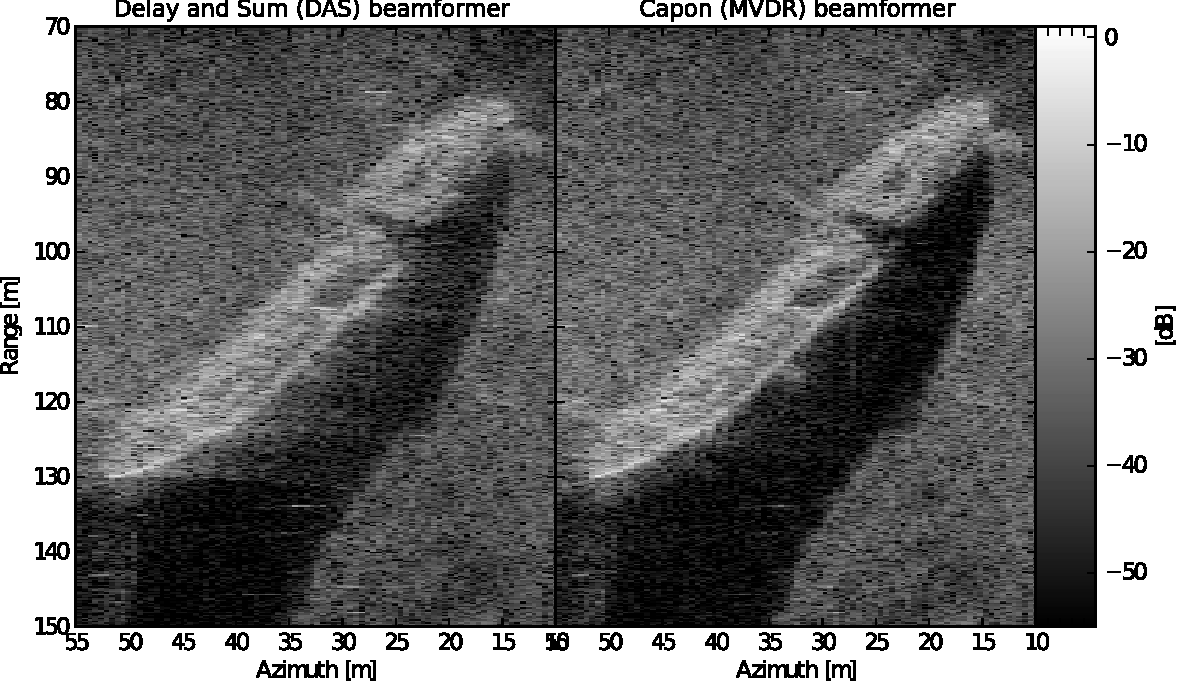
\includegraphics[width=\linewidth]{gfx/img_holmengraa.ps}
\caption{HISAS sidescan sonar (SSS) image of the shipwreck Holmengraa.}\label{holmengraa}
\end{figure}

We have tested our \gls{GPU} implementation of the \gls{MVDR} beamformer on two different experimental datasets from the 32 element Kongsberg Maritime HISAS1030 sonar~\cite{Hansen2009}. The sonar was attached to the HUGIN \gls{AUV}, and was in one of the datasets used in sidescan mode to image the 1500 dwt oil tanker wreck Holmengraa (\Fig{holmengraa}). Holmengraa is roughly 68\,m long and 9\,m wide, and lies on a slanted seabed at 77\,m depth. The \gls{MVDR} image was created with the parameters $L=16$, $N_\text{avg}=3$, and $d=1\%$, which proved to be a reasonable selection for this scenario.

The other dataset was a 55\,kpixel sectorscan test image. We used it to benchmark our \gls{MVDR} implementation, and compared the result with the runtimes of an optimized single-thread C and Matlab implementation (\Fig{benchmarks}). Processing times are shown for varying subarray lengths $L$ and varying amounts of temporal averaging $N_\text{avg}$. The test system was a quad-core Intel Xeon E5620, with 64Gb of \gls{RAM}, and an nVidia Quadro 6000 card. This is a \gls{GPU} with 448 \gls{CUDA} cores and 6Gb of onboard \gls{RAM}, capable of performing roughly 1Tflops.

\section{Discussion}

Figure \ref{holmengraa} demonstrates the \gls{MVDR} beamformer's ability to suppress interference and achieve better detail resolution. Compared the \gls{DAS} beamformer, the ship's edges come out as sharper, and the shadows are less noisy. But while \gls{DAS} processed this 1.3\,Mpixel image in milliseconds, our Matlab implementation\todo{never mentioned matlab vefore} of MVDR beamformer needed minutes.

As Figure \ref{benchmarks} illustrates, using a \gls{GPU} improves matters. If we look at the total runtimes for a subarray size of $L=16$ and temporal averaging at $K=2$, the \gls{GPU} implementation is able to process the test image in roughly 40\,ms. This translates to a processing throughput of 1.4\,Mpixels/s. For the same scenario the C implementation clocked in at roughly 3\,s and Matlab at 17\,s, which is 75 and 435 times slower than the \gls{GPU} implementation, respectively.

Interesting to note is also that solving $\eRi\1$ remains the main bottleneck in the \gls{GPU} implementation, and it gets even worse for larger $L$'s. However, this is a general Gauss Jordan solver which does not exploit symmetry properties of $\eR$, so creating e.g.\ a batch based Cholesky solver should improve the runtimes further. Both the C and Matlab implementation in this benchmark take this symmetry into account, which partially explains why the complexity curves of these implementations are different from that of the \gls{GPU} implementation.

\begin{figure}[t]
\centering
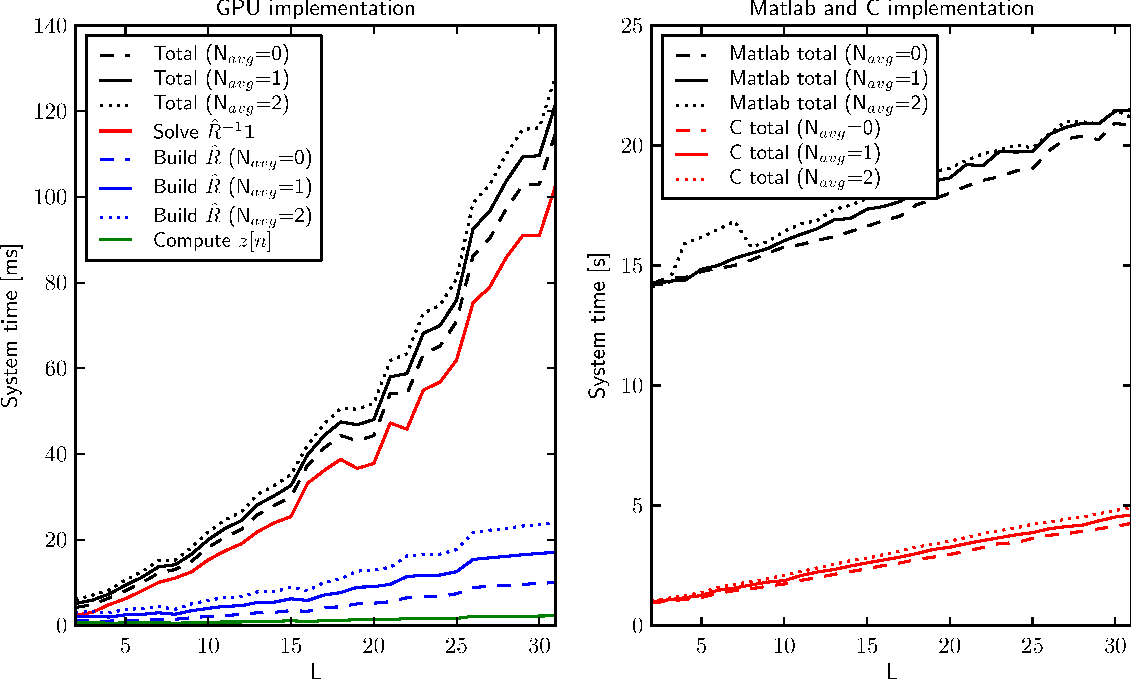
\includegraphics[width=\linewidth]{gfx/benchmark.ps}
\caption{\protect\gls{MVDR} benchmarks. Forming a 55\,kpixel image from a $M=32$ channel array.}\label{benchmarks}
\end{figure}

If the HISAS1030 was attached to a platform moving at 1.8m/s, for which the maximum range is 250\,m~\cite{Hansen2010}, the pulse repetition frequency could be set to 3\,Hz. We further assume a critical complex sampling frequency equal to the HISAS1030's bandwidth of 30\,kHz, and beamform $M=32$ lateral beams. The throughput required for realtime processing of these images would then be 1\,Mpixels/s. As we have seen, this is something our \gls{GPU} implementation can handle if $L$ is not too large.%, leaving the \gls{CPU} free to take on other assignments.





% - Sidescan: 40kHz 

What may this performance be used for? Let us assume that the 32 element, 1.2\,m long HISAS1030 array is mounted on a platform moving at 1.8\,m/s. Then the pulse repetition frequency (PRF) could be set to 3\,Hz to ensure critical along-track sampling, 
To illustrate what this performance might be used for, consider a moving platform travelling at 1.8\,m/s. 
If the sonar system is Maximum range 
There is a limit to the along-track sampli
To avoid along track undersampling, the 



% HUGIN: 1.8m/s - range 250m \\
% fs = 100kHz*30\%*$\frac{4}{3}$ = 40kHz \\
% $N_{range px} = \frac{2\,250m}{1500m/s}40kHz = 13.3kpx$ \\
% $\times 32$ beams = 426kpx \\\\
% 
% PRF = $\frac{1500m/s}{2 250m} = 3Hz$ \\
% TP = 215px 3Hz = 1.28Mpx/s \\
% 4 arrays: 1.28Mpx/s * 4 = 5.12Mpx/s
% 
% 
% \begin{itemize}
% \item Need for speed: HUGIN 4 banks of 32 elements, can be processed faster than the ping repetition rate, with margins to spare.
% \end{itemize}


\section{Conclusion}

The \gls{MVDR} beamformer is an algorithm well suited for implementation on a \gls{GPU}. This is because the computations involved are independent on a pixel level, and partially also within each pixel. We were able to achieve speedup factors of 2-3 orders of magnitude by implementing our active sonar capable \gls{MVDR} implementation on a high-end \gls{GPU}. This performance is sufficient for computing critically sampled full-coverage sectorsscan images from the HISAS1030 sonar in realtime. Furthermore, even if such processing speeds are not required, it might be advantageous to relieve the \gls{CPU} from some of its workload. After all, these chips were designed to cooperate.

\begin{figure}[t]
\centering
\includegraphics[width=\linewidth]{gfx/benchmark_tagged.eps}
\caption{Realtime requirement for sectorscan imaging.}\label{realtime_sectorscan}
\end{figure}

%%%%%%%%%%%%%%%%%%                              ~~~~~~~~~~~~~~~~~~~~~~~~~~~~~~~~~~~~~~~~~~~~~~~~~~
% DOCUMENT APPENDICES %
%%%%%%%%%%%%%%%%%%                              ~~~~~~~~~~~~~~~~~~~~~~~~~~~~~~~~~~~~~~~~~~~~~~~~~~


% \titleformat{<command>}[<shape>]{<format}{<label>}{<sep>}{<before>}[<after>]

% \titleformat{\section}[hang]{\bf}
% {\thesection.\enspace}%\thesubsubsection}%  {\footnotesize \enspace \emph{Sec.}  }
%    {0pt}{\MakeUppercase}[]
% \titlespacing*{\section}{0pt}{2\lineheight}{\lineheight}

% {-2ex plus -.5ex minus -.2ex}{1.0ex plus .2ex minus .2ex}

% \renewcommand\section[1]{{\Large\bf\MakeUppercase #1}}
% \renewcommand\section*[1]{{\Large\bf\MakeUppercase #1}}

% 
% 
% 
% 
% 
% 
% \section{Introduction}
% 
% \todopar{Case:
% \begin{itemize}
% \item UFFC(?)
% \item Ultrasound. Arrays up to 128 channels. Processing power vital. What's the best way to implement 
% \item Other articles evaluates Capon image quality, and some have shown that speedups can be achieved by reducing the complexity of the traditional Capon algorithm or by implementing specific versions on a GPU.
% \item This article compare a few promising ways to implement Capon in general, in light of general complexity and suitability for implementation on a CPU and GPU.
% \end{itemize}
% }
% 
% \begin{itemize}
% \item As briefly as possible, introduce beamforming.
% \item Adaptive beamformer's potential lies in its ability to suppress interference power
% \item Why adaptive beamformers struggle in active sonar systems. Correlated noise, robustification kills the adaptive potential. Quite computationally intensive. Constraints must be applied in one way or another - parameters must be tuned.
% \item The three main ways to implement Capon \cite{Capon1969} is \todo{not entirely true?}
% \begin{itemize}
% \item Traditional way: Build $\eR$ and solve $\w = \frac{\Ri\a}{\a\H\Ri\a}$. 
% \item Iterative methods: Woodbury, Conjugated gradients
% \item Beamspace
% \item LCA (or other methods, as reference)
% \end{itemize}
% \item Choice of robustification parameters $L,M,\Delta$ largely impacts what the ``optimal'' way of implementing Capon 
% \item In most imaging applications 
% Outline:
% \begin{itemize}
% \item Speeding up: Build $\eR$ and solve $\w = \frac{\Ri\a}{\a\H\Ri\a}$. 
% \item Iterative methods: Woodbury (Sherman Morrison), Conjugated gradients - show performance of GPU performance.
% \item Woodbury: Must take the average over many samples in space and time - lots of (small) outerproducts. Can be used if not a lot of averaging is required.
% \item Beamspace
% \item LCA (or other methods, as reference)
% \end{itemize}
% \end{itemize}
% 
% fs = 100kHz*30\%*$\frac{4}{3}$ = 40kHz \\
% $N_{range px} = \frac{2\,250m}{1500m/s}40kHz = 13.3kpx$ \\
% $\times 32$ beams = 426kpx \\\\
% 
% PRF = $\frac{1500m/s}{2 250m} = 3Hz$ \\
% TP = 215px 3Hz = 1.28Mpx/s \\
% 4 arrays: 1.28Mpx/s * 4 = 5.12Mpx/s
% 
% 
% \section{Methods}
% 
% \begin{align}
% z[n] = \sumb{m=0}{M-1} w_m[n]^*x_m[n-\Delta_m] = \w\H[n]\Xd[n]
% \end{align}
% where
% \begin{align}
% \w[n] = \bmat{w_0[n]\\w_1[n]\\\vdots\\w_{M-1}[n]} \quad \text{and} \quad\Xd[n] = \bmat{x_0[n]\\x_1[n]\\\vdots\\x_{M-1}[n]}.
% \end{align}
% 
% Minimum variance distortionless resonse \cite{Capon1969}
% \begin{align}
% \underset{\w[n]}{\argmin}\, E\{ |z[n]|^2 \} = \underset{\w[n]}{\argmin}\, \w\H[n]\R[n]\w[n], 
% \end{align}
% subject to
% \begin{align}
% \w\H[n]\a = 1,
% \end{align}
% where
% \begin{align}
% \R[n] = E\{ \x\x\H \}.
% \end{align}
% If $\eR$ is the estimate of $\R$, the solution to the MVDR beamformer is
% \begin{gather*}
% \vec w[n] = \frac{\hat{\mat R}\,\!^{-1}[n]\vec a}{\vec a\H\hat{\mat R}\,\!^{-1}[n]\vec a} = \frac{\text{\raisebox{1.9pt}{$\vec\chi$}}[n]}{\vec a\H\text{\raisebox{1.9pt}{$\vec\chi$}}[n]}
% \end{gather*}
% A robust estimate of $\eR$ is found by
% \begin{itemize}
% \item Spatial averaging to decorrelate noise from signal. \emph{Subarray averaging} used here.
% \item Temporal averaging to ensure valid speckle statistics.
% \item \emph{Diagonal loading} to ensure  numerical stability prior to inversion.
% \item Choice of robustification parameters \cite{Synnevag2007}
% \end{itemize}
% 


\newpage

\appendix[Throughput]

{\bf Method complexity (instructions):}\\
\begin{tabular}{l l}
No optimizations            & $2M^2\,(2\Navg+1)$ \\
Banded symmetric            & $L(2M-L+1)\,(2\Navg+1)$ \\
Sliding, banded, symmetric  & $1.5L(2M-L+1)$ \\
\end{tabular}\\\\

{\bf Number of complex numbers needed per SM when building R:}\\
\begin{align*}
\left\lfloor\frac{T_b}{L}\right\rfloor(M+L)+2MN
\end{align*}

% Is the method compute bound, memory throughput bound, or memory latency bound?
% 
% Take as example the case in Fig \ref{mvdr_complexity} in case where $M=32$, $L=16$ and $K=1$. The figure shows a that 300k floating point operations need to be performed per pixel. Furthermore, the total size of global reads is $(M+L)*8$bytes$ = 96$floats per px, and the total number of writes is $L^2*2$floats = 512 floats, leading to a total of 608 floats. This means that roughly 1000 arithmetic instructions are carried for every 0.6 float transferred from or to global memory.
% 
% If an algorithm is neither bandwidth bound or computationally bound, it might be bound by latency. 
% 
% 
% 1Tflops (ops/cycle?)
% 144GB/s global
% 1TB/s shared
% x6 regs
% 
% latency - arithmethic (20 cycles) and memory (400+ cycles)
% 
% Little's law - needed parallelism = latency * throughput
% arithmetic: 23 cycles * 32ops/SM/cycle = 576 ops/SM parallelism
% memory: <800 cycles * <144GB/s=125B/cycle = <100kB in the flight
% 
% On GF104: must have some ILP to get >0.66 of peak:
% - 48cores/SM, one instruction is broadcast across 16 cores
% - need 3 instructions per cycle
% - but only have 2 warp schedulers
% - instead, can issue 2 instructions per warp in the same cycle
% 
% 
% need to compute op/float ratios
% non-optimized: M=32,L=16, 300kops/px / 40k floats/px = 8 ops/float. op bound if shared is used
% optimized: 50kops/px / 40k floats/px = 1 ops/float. memm bound even if shared is used. some ilp advantageous

\appendix{Arithmetic Throughput and Memory Throughput}\label{throughput}

In the context of determining whether an implementation is computationally bound or memory bound, one should first compare the target platform's sustained computational throughput to sustained memory throughput. Let us start with the former.

The Quadro 6000 has 32 CUDA cores per SM, each operating at a rate of 1\,148\,MHz and being able to perform 2 floating point operations (flop) per clock cycle. Theoretical peak arithmethic throughput is then given as:
\begin{align}
\text{BW}_\text{arithmethic} &= 2\cdot1\,148\,\text{flop/s/core}\cdot 32\,\text{cores/SM}\cdot 14\,\text{SMs}\nn
&= 1.03\,\text{Tflop/s}.\label{flops}
\end{align}
Now let us compare this to the memory throughput. The ``global'' GDDR5 memory bus is 384\,bit wide, and operates at 3\,Ghz where 2 bits are sent every cycle. Its peak bandwidth is then:
\begin{align}
\text{BW}_\text{global} &= \frac{2\cdot 3\,\text{Gbit/s}\cdot384\,\text{bit}}{8\,\text{bit/byte}}\nn
&= 144\,\text{GB/s}\ (36\,\text{Gfloats/s}).\label{bwglobal}
\end{align}
The shared memory, on the other hand, are organized into 32 banks per SM, each being 32\,bit wide and operating at 1\,148\,MHz where 1 bit is sent per cycle. Its peak aggregated bandwidth is then:
\begin{align}
\text{BW}_\text{shared} &= \frac{\frac{1\,148}{2}\,\text{Mbit/s}\cdot32\,\text{bit/bank}\cdot 32\,\text{banks/SM}\cdot 14\,\text{SMs}}{8\,\text{bit/byte}}\nn
&\approx 1.03\,\text{TB/s}\ (257\,\text{Gfloats/s}).\label{bwshared}
\end{align}
The bandwidths are compared in Tab. \ref{tabbandwidth}. Note that even when using shared memory at least 4 floating point operations must be carried out per float transferred to the CUDA cores, otherwise the algorithm with be memory bound. In such cases instruction level parallelism can be exploited to move data from shared memory into the even faster register memory~\cite{Vasilyy}, but this is outside the scope of this article.


% 
% \subsubsection{Computing $\text{\raisebox{1.9pt}{$\vec\chi$}} = \hat{\mat R}\,\!^{-1}\vec a$}
% 
% There are two ways of finding $\text{\raisebox{1.9pt}{$\vec\chi$}} = \hat{\mat R}\,\!^{-1}\vec a$, either by solving the equation directly or by inverting $\hat{\mat R}$ first. Solving the equation is less computationally intensive than inverting $\hat{\mat R}$, and seems like the obvious choice. However, with iterative methods for updating $\eRi$ for each range pixel the situation is changed...

% 
% \subsection{Iterative methods}
% 
% \begin{itemize}
% \item Woodbury
% \item Conjugated gradients
% \end{itemize}
% 
% 
% \subsection{Beamspace}
% 
% \begin{itemize}
% \item Some minimum of background, and good references.
% \end{itemize}
% 
% 
% \section{Results/Discussion}
% 
% 
% 
% 
% 
% \begin{itemize}
% \item Compare computational complexity vs. memory constraints for the various methods. Supporting plots.
% \item Relate this to whether the favourable architecture is a CPU or a GPU \todo{check ``when to gpu article''}
% \item Run benchmarks on some sonar dataset(s)
% \end{itemize}
% 
% 
% \section{Conclusion}
% 
% \begin{itemize}
% \item When to use what.
% \end{itemize}
% 
% 
% % \ \\
% % \IEEEPARstart{T}{o} form images from a modern phased array sonar system the received wavefield is usually recorded, and then postprocessed by a digital beamformer. The beamformer applies delays and weights to the sensor channels, the beamformer adjusts the arrays spatial response to focus at one pixel at a time.  such that signals emanating from regions of interest add constructively, while ensuring that noise and interference from other angles do not. 
% % 
% % The imaging capabilities of a modern phased array sonar system depend on physical attributes such element response and array geometry, the transmitted signal, as well as the beamforming method being used on transmission and reception. Beamforming is the concept of applying delays and weights to the sensors channels to steer the arrays response to points of interest. 
% 
% % 
% % 
% % Outline:
% % \begin{itemize}
% % \item Capon's resonse when applying robustification
% % \item Choice of window functions makes little difference.
% % \item Steering and mainlobewidths have outer bounds.
% % \item Beamspace?
% % \item Chosen window plots - what may they tell us? Variance intensity values when using various windows.
% % \item Assymmetric windows?
% % \end{itemize}
% % 
% % 
% % \begin{align}
% % z[n] = \sumb{m=0}{M-1} w_m[n]^*x_m[n-\Delta_m] = \w\H[n]\x[n-\Delta_m]
% % \end{align}
% % 
% % 
% % \section{Methods}
% % 
% % Basically, we are working with a practical implementation of the Capon beamformer that computes a set of weights $\vec w$ for every single sample $n$ by solving:
% % \begin{gather*}
% % \vec w[n] = \frac{\hat{\mat R}\,\!^{-1}[n]\vec a}{\vec a\H\hat{\mat R}\,\!^{-1}[n]\vec a} = \frac{\text{\raisebox{1.9pt}{$\vec\chi$}}[n]}{\vec a\H\text{\raisebox{1.9pt}{$\vec\chi$}}[n]}
% % \end{gather*}%
% % where
% % % \newcommand\X{\text{\raisebox{2pt}{$\vec\chi$}}}
% % \begin{gather*}
% % \text{\raisebox{1.9pt}{$\vec\chi$}} = \hat{\mat R}\,\!^{-1}\vec a \qquad\qquad\text{is the solution to}\qquad\qquad \hat{\mat R}\text{\raisebox{1.9pt}{$\vec\chi$}} = \vec a.
% % \end{gather*}
% 
% % 
% % , and maximum suppression of while ensuring that the beamformer digitally  before each of the pixels are estimated one at a time. The resolution and contrast of such a system will depend on the systems spatial response, which ideally should be narrow  be very sharp in the desired direction its ability to achieve  fundamental principle of forming a sonar image is to record the received wavefield, 
% % 
% % image quality of a phased array sonar imaging systems depend on  the choice of weights to apply to each of the sensors are crucial. 
% % 
% % A modern phased array imaging system may be thought of as a spatial filter. To achieve the best possible performance, the 
% % 
% % resolution and contrast 
% % 
% % Adaptive beamformers have only recently been introduced in active sonar imaging. For a while they were considered unsuited for this purpose because the backscattered signal is largely correlated with the 
% % 
% % 
% % 
% 
% %\begin{figure}[!t]
% %\centering
% %\includegraphics[width=2.5in]{myfigure}
% % where an .eps filename suffix will be assumed under latex, 
% % and a .pdf suffix will be assumed for pdflatex; or what has been declared
% % via \DeclareGraphicsExtensions.
% %\caption{Simulation Results}
% %\label{fig_sim}
% %\end{figure}
% 
% 
% % An example of a double column floating figure using two subfigures.
% % (The subfig.sty package must be loaded for this to work.)
% % The subfigure \label commands are set within each subfloat command, the
% % \label for the overall figure must come after \caption.
% % \hfil must be used as a separator to get equal spacing.
% % The subfigure.sty package works much the same way, except \subfigure is
% % used instead of \subfloat.
% %
% % \begin{figure*}[!t]
% % \centerline{\subfloat[Case I]\includegraphics[width=2.5in]{subfigcase1}%
% % \label{fig_first_case}}
% % \hfil
% % \subfloat[Case II]{\includegraphics[width=2.5in]{subfigcase2}%
% % \label{fig_second_case}}}
% % \caption{Simulation results}
% % \label{fig_sim}
% % \end{figure*}
% %
% % Note that often IEEE papers with subfigures do not employ subfigure
% % captions (using the optional argument to \subfloat), but instead will
% % reference/describe all of them (a), (b), etc., within the main caption.
% 
% 
% % An example of a floating table. Note that, for IEEE style tables, the 
% % \caption command should come BEFORE the table. Table text will default to
% % \footnotesize as IEEE normally uses this smaller font for tables.
% % The \label must come after \caption as always.
% %
% %\begin{table}[!t]
% %% increase table row spacing, adjust to taste
% %\renewcommand{\arraystretch}{1.3}
% % if using array.sty, it might be a good idea to tweak the value of
% % \extrarowheight as needed to properly center the text within the cells
% %\caption{An Example of a Table}
% %\label{table_example}
% %\centering
% %% Some packages, such as MDW tools, offer better commands for making tables
% %% than the plain LaTeX2e tabular which is used here.
% %\begin{tabular}{|c||c|}
% %\hline
% %One & Two\\
% %\hline
% %Three & Four\\
% %\hline
% %\end{tabular}
% %\end{table}
% 
% 
% % Note that IEEE does not put floats in the very first column - or typically
% % anywhere on the first page for that matter. Also, in-text middle ("here")
% % positioning is not used. Most IEEE journals use top floats exclusively.
% % However, Computer Society journals sometimes do use bottom floats - bear
% % this in mind when choosing appropriate optional arguments for the
% % figure/table environments.
% % Note that, LaTeX2e, unlike IEEE journals, places footnotes above bottom
% % floats. This can be corrected via the \fnbelowfloat command of the
% % stfloats package.
% 
% 
% 
% \section{Conclusion}
% The conclusion goes here.
% 
% 
% 


% if have a single appendix:
%\appendix[Proof of the Zonklar Equations]
% or
%\appendix  % for no appendix heading
% do not use \section anymore after \appendix, only \section*
% is possibly needed

% use appendices with more than one appendix
% then use \section to start each appendix
% you must declare a \section before using any
% \subsection or using \label (\appendices by itself
% starts a section numbered zero.)
%

%%%%%%%%%%%%%%%%%%                              ~~~~~~~~~~~~~~~~~~~~~~~~~~~~~~~~~~~~~~~~~~~~~~~~~~
% DOCUMENT APPENDICES %
%%%%%%%%%%%%%%%%%%                              ~~~~~~~~~~~~~~~~~~~~~~~~~~~~~~~~~~~~~~~~~~~~~~~~~~

\appendices



% use section* for acknowledgement
\ifCLASSOPTIONcompsoc
  \section*{Acknowledgments}
\else
  \section*{Acknowledgment}
\fi


The authors would like to thank Nvidia\todo{drop this now that the batch solver is official?} for providing them their unofficial linear equation batch solver, and Kongsberg Maritime and the Norwegian Defence Research Establishment (FFI) for providing experimental data.


% Can use something like this to put references on a page
% by themselves when using endfloat and the captionsoff option.
\ifCLASSOPTIONcaptionsoff
  \newpage
\fi



% trigger a \newpage just before the given reference
% number - used to balance the columns on the last page
% adjust value as needed - may need to be readjusted if
% the document is modified later
%\IEEEtriggeratref{8}
% The "triggered" command can be changed if desired:
%\IEEEtriggercmd{\enlargethispage{-5in}}

% references section

\bibliographystyle{IEEEtran}
\bibliography{../../Library/library}

% End up doing this:
% \begin{thebibliography}{1}
% 
% \bibitem{IEEEhowto:kopka}
% H.~Kopka and P.~W. Daly, \emph{A Guide to {\LaTeX}}, 3rd~ed.\hskip 1em plus
%   0.5em minus 0.4em\relax Harlow, England: Addison-Wesley, 1999.
% 
% \end{thebibliography}



% biography section
% 
% If you have an EPS/PDF photo (graphicx package needed) extra braces are
% needed around the contents of the optional argument to biography to prevent
% the LaTeX parser from getting confused when it sees the complicated
% \includegraphics command within an optional argument. (You could create
% your own custom macro containing the \includegraphics command to make things
% simpler here.)
%\begin{biography}[{\includegraphics[width=1in,height=1.25in,clip,keepaspectratio]{mshell}}]{Michael Shell}
% or if you just want to reserve a space for a photo:

\vfill 

\begin{IEEEbiography}{Noname dude}
He doesn't exist.
\end{IEEEbiography}

% if you will not have a photo at all:
\begin{IEEEbiographynophoto}{Jo Inge Buskenes}
Not in at the moment.
\end{IEEEbiographynophoto}

%\newpage

% \begin{IEEEbiographynophoto}{Jo Inge Buskenes}
% Not in at the moment.
% \end{IEEEbiographynophoto}

%\vfill

% Can be used to pull up biographies so that the bottom of the last one
% is flush with the other column.
%\enlargethispage{-5in}

\markboth{}%
{}
% \newpage
\begin{figure*}[!t]
\begin{narrow}{-1.2cm}{-1.2cm}\centering\vspace{-1.0cm}
\textbf{1. LCA with trigonometric and Kaiser windows - Capon shining}\\
\begin{tabular}[c]{l l l l}
\bf General & M = 32                            & $\Delta r = \frac{c}{2B}$ = 2.5 cm & $\frac{640\,\text{pixels}] / 12\,\text{m}}{\Delta r} = \frac{4}{3}$ \\
\bf LCA     & $\beta \in [0,10]$ (9 values) & $\phi \in [-1.07,1.07]$ deg (9 values) & Navg = 3 \\
\bf Capon   & $\Delta$ = 0.01                 & L = 16                           & Navg = 3 \\
\end{tabular}
\subfloat[LCA Window Response]{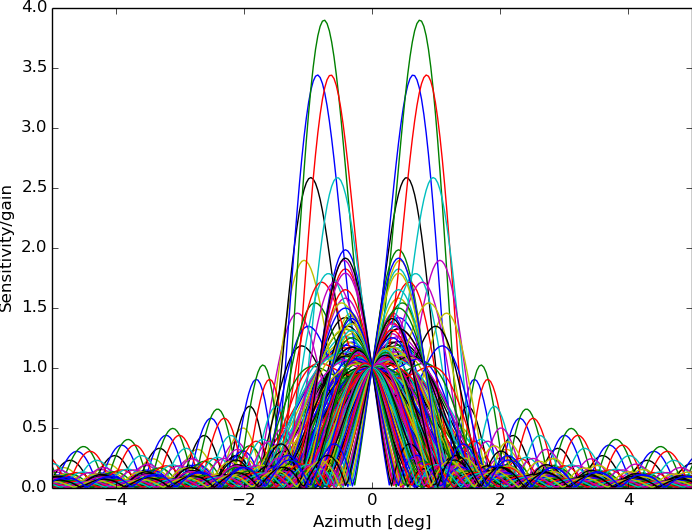
\includegraphics[width=0.49\linewidth]{gfx/1_window_response.png}}\hfill
\subfloat[Mean images]{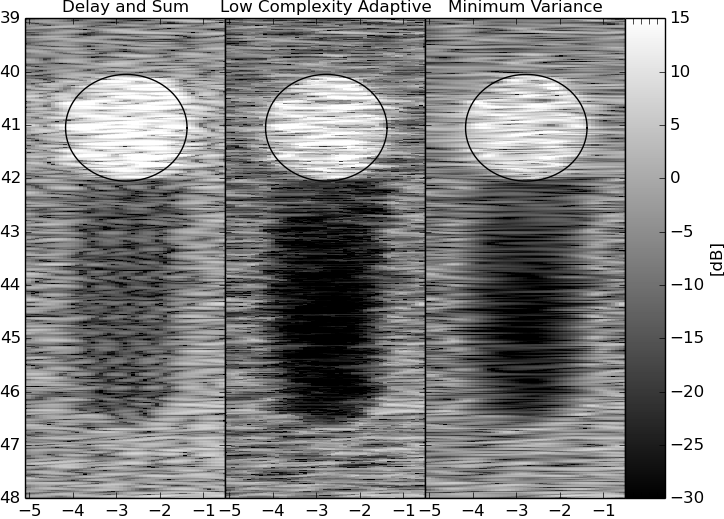
\includegraphics[width=0.49\linewidth]{gfx/1_mean_imgs.png}}\\
\subfloat[Windows ($\beta$)]{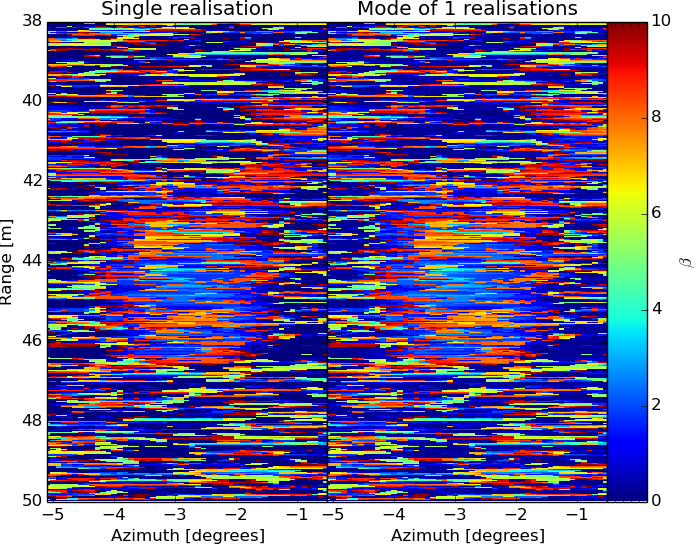
\includegraphics[width=0.49\linewidth]{gfx/1_windows_beta.png}}\hfill
\subfloat[Windows ($\phi$)]{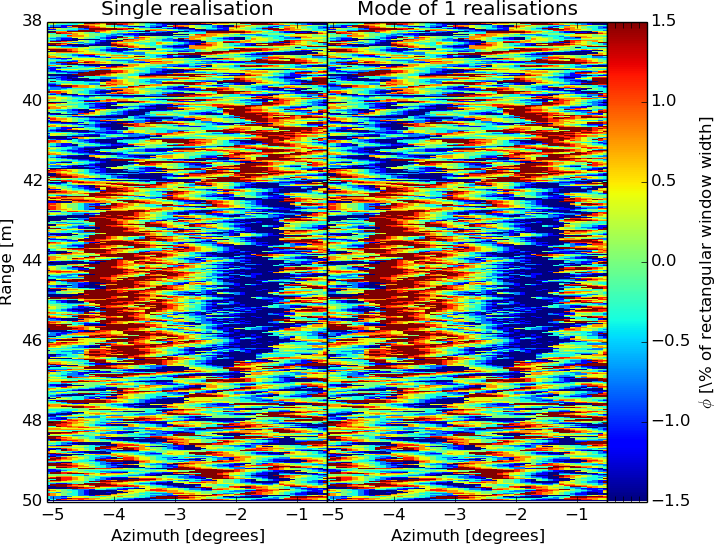
\includegraphics[width=0.48\linewidth]{gfx/1_windows_phi.png}}\\
\subfloat[Capon win. resp. through shadow]{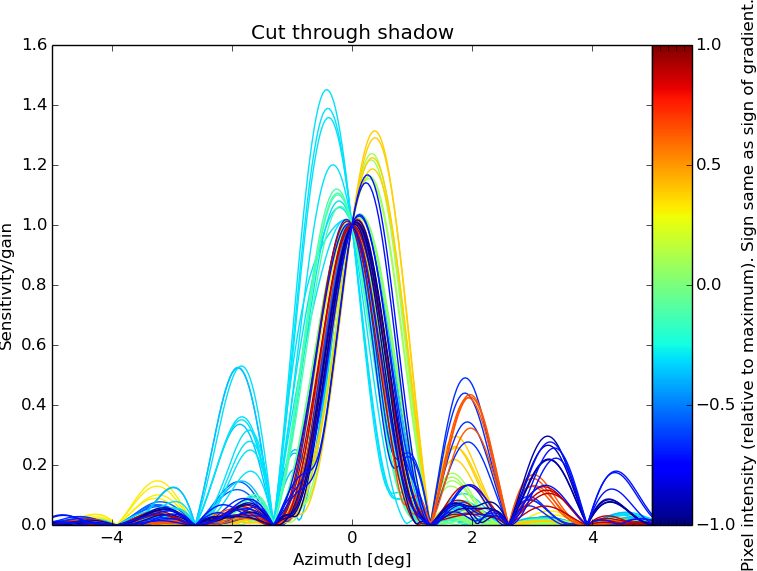
\includegraphics[width=0.49\linewidth]{gfx/1_win_resp_cut_shadow.png}}\hfill
\subfloat[Capon win. resp. through highlight]{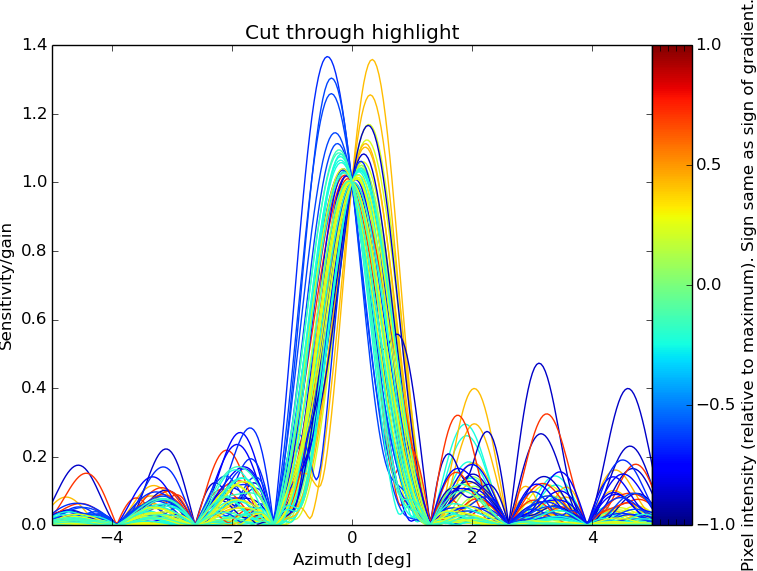
\includegraphics[width=0.49\linewidth]{gfx/1_win_resp_cut_highlight.png}}\\
\end{narrow}
\end{figure*}
\newpage
\begin{figure*}[!t]
\begin{narrow}{-1.2cm}{-1.2cm}\centering\vspace{-1.0cm}
\textbf{2. Capon: Tuning regularisation.}\\
\begin{tabular}[c]{l l l l}
\bf General & M = 32                            & $\Delta r = \frac{c}{2B}$ = 2.5 cm & $\frac{640\,\text{pixels}] / 12\,\text{m}}{\Delta r} = \frac{4}{3}$ \\
\bf LCA     & $\beta \in [0,10]$ (9 values) & $\phi \in [-1.07,1.07]$ deg (9 values) & Navg = 3 \\
\bf Capon   & $\Delta$ = 0.05                 & L = 16                           & Navg = 3 \\
\end{tabular}
\subfloat[LCA Window Response]{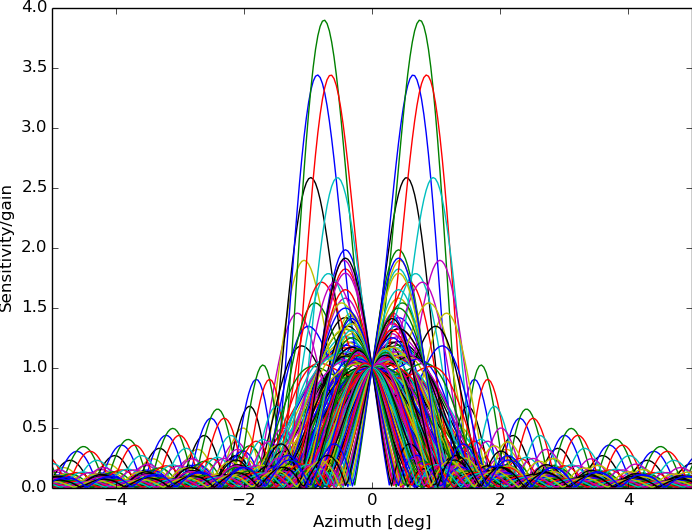
\includegraphics[width=0.49\linewidth]{gfx/2_window_response.png}}\hfill
\subfloat[Mean images]{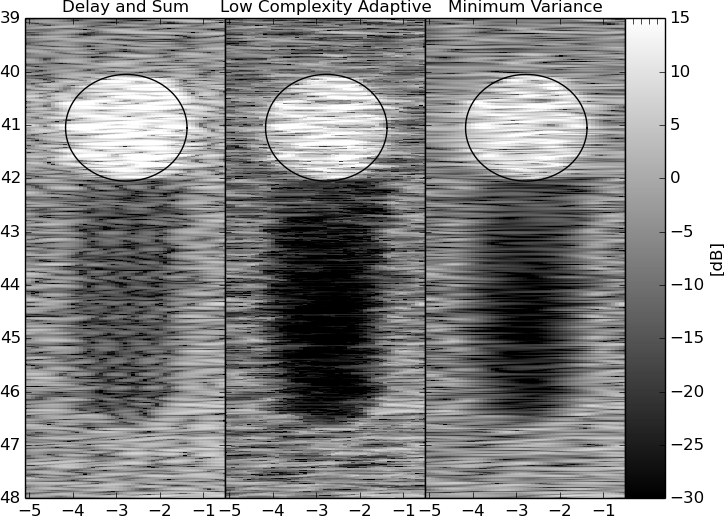
\includegraphics[width=0.49\linewidth]{gfx/2_mean_imgs.png}}\\
\subfloat[Windows ($\beta$)]{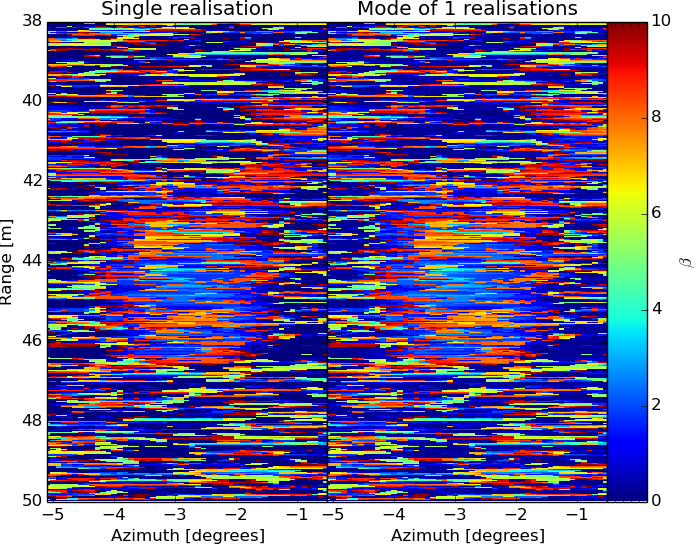
\includegraphics[width=0.49\linewidth]{gfx/2_windows_beta.png}}\hfill
\subfloat[Windows ($\phi$)]{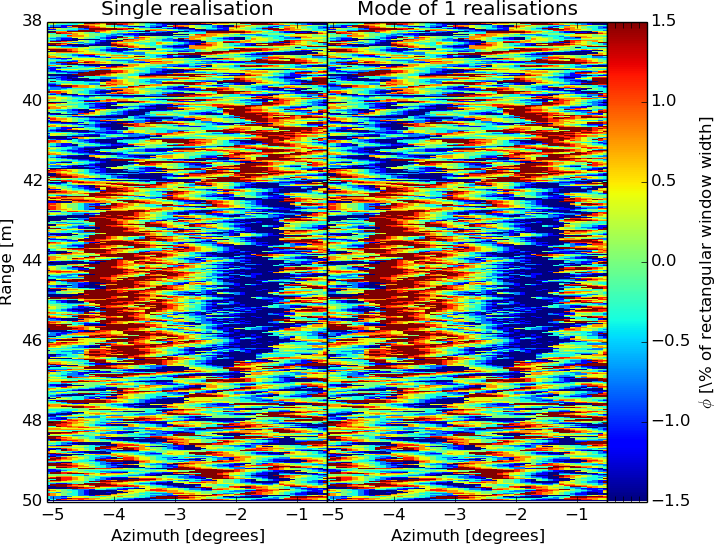
\includegraphics[width=0.48\linewidth]{gfx/2_windows_phi.png}}\\
\subfloat[Capon win. resp. through shadow]{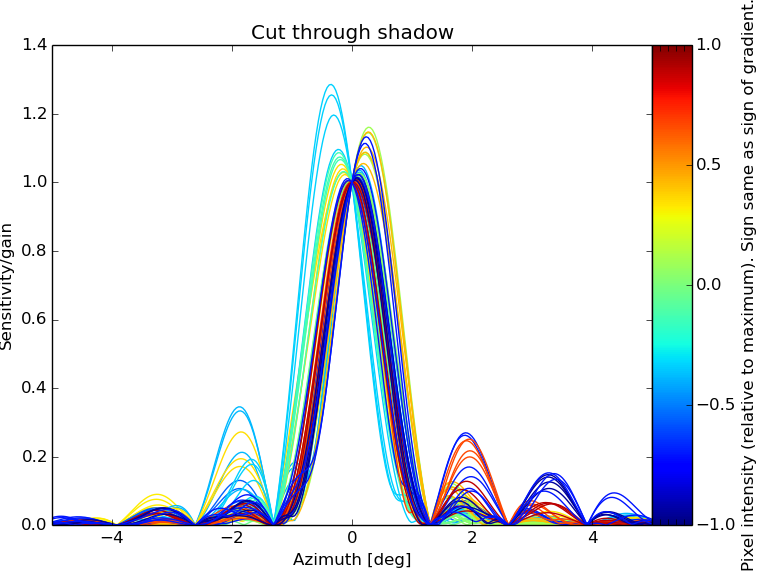
\includegraphics[width=0.49\linewidth]{gfx/2_win_resp_cut_shadow.png}}\hfill
\subfloat[Capon win. resp. through highlight]{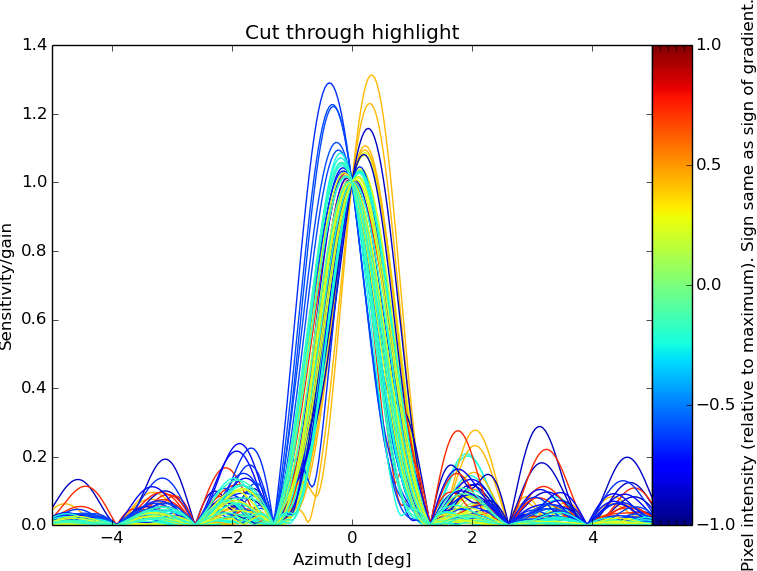
\includegraphics[width=0.49\linewidth]{gfx/2_win_resp_cut_highlight.png}}\\
\end{narrow}
\end{figure*}
\newpage
\begin{figure*}[!t]
\begin{narrow}{-1.2cm}{-1.2cm}\centering\vspace{-1.0cm}
\textbf{3. Capon: Tuning regularisation.}\\
\begin{tabular}[c]{l l l l}
\bf General & M = 32                            & $\Delta r = \frac{c}{2B}$ = 2.5 cm & $\frac{640\,\text{pixels}] / 12\,\text{m}}{\Delta r} = \frac{4}{3}$ \\
\bf LCA     & $\beta \in [0,10]$ (9 values) & $\phi \in [-1.07,1.07]$ deg (9 values) & Navg = 3 \\
\bf Capon   & $\Delta$ = 0.20                 & L = 16                           & Navg = 3 \\
\end{tabular}
\subfloat[LCA Window Response]{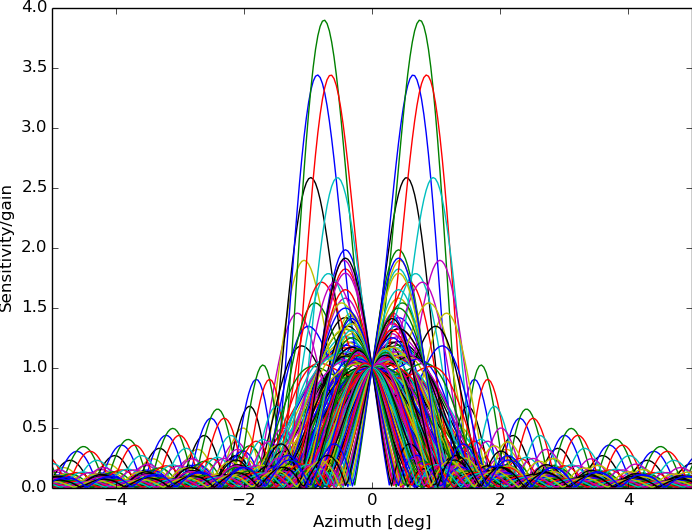
\includegraphics[width=0.49\linewidth]{gfx/3_window_response.png}}\hfill
\subfloat[Mean images]{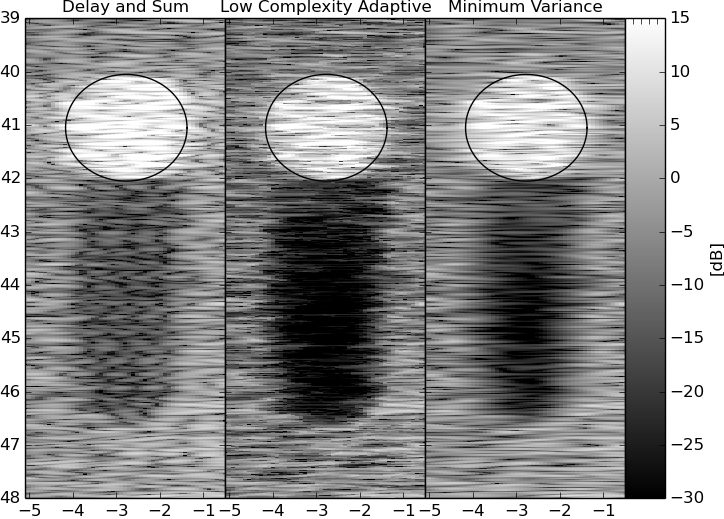
\includegraphics[width=0.49\linewidth]{gfx/3_mean_imgs.png}}\\
\subfloat[Windows ($\beta$)]{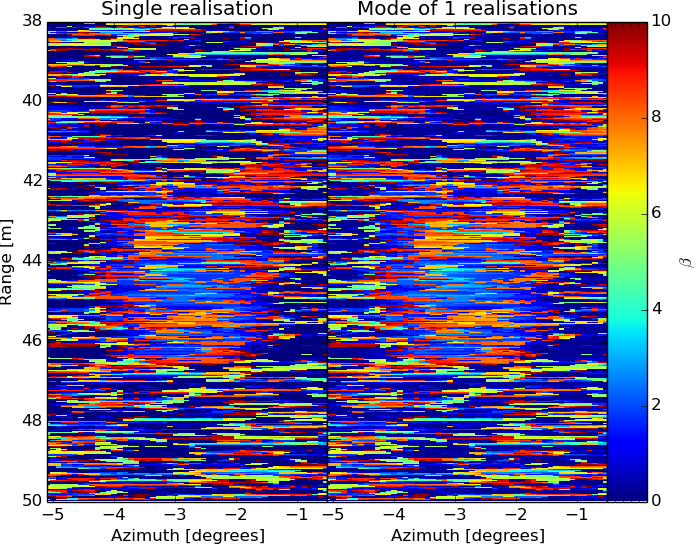
\includegraphics[width=0.49\linewidth]{gfx/3_windows_beta.png}}\hfill
\subfloat[Windows ($\phi$)]{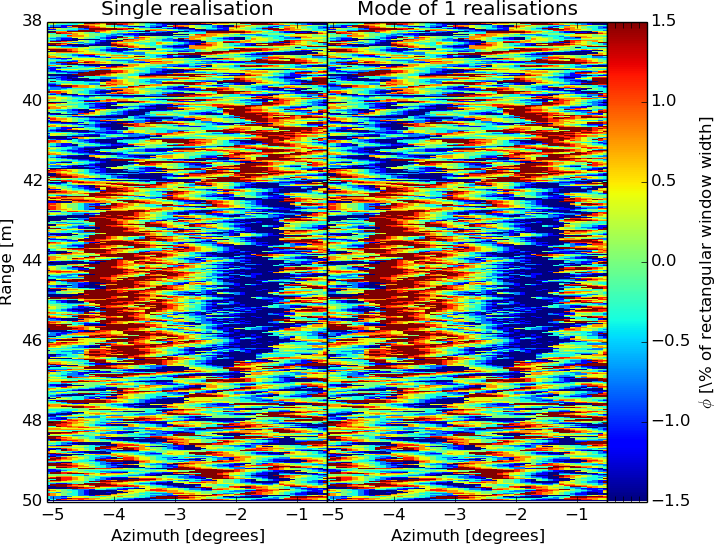
\includegraphics[width=0.48\linewidth]{gfx/3_windows_phi.png}}\\
\subfloat[Capon win. resp. through shadow]{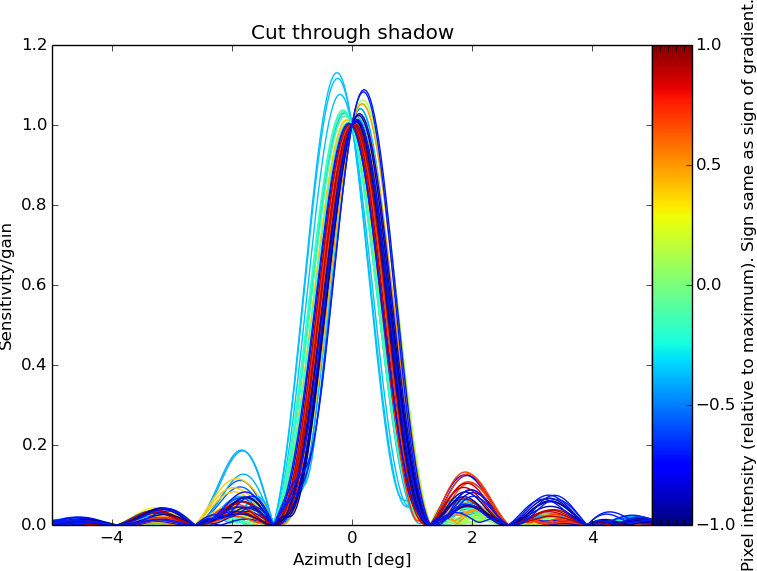
\includegraphics[width=0.49\linewidth]{gfx/3_win_resp_cut_shadow.png}}\hfill
\subfloat[Capon win. resp. through highlight]{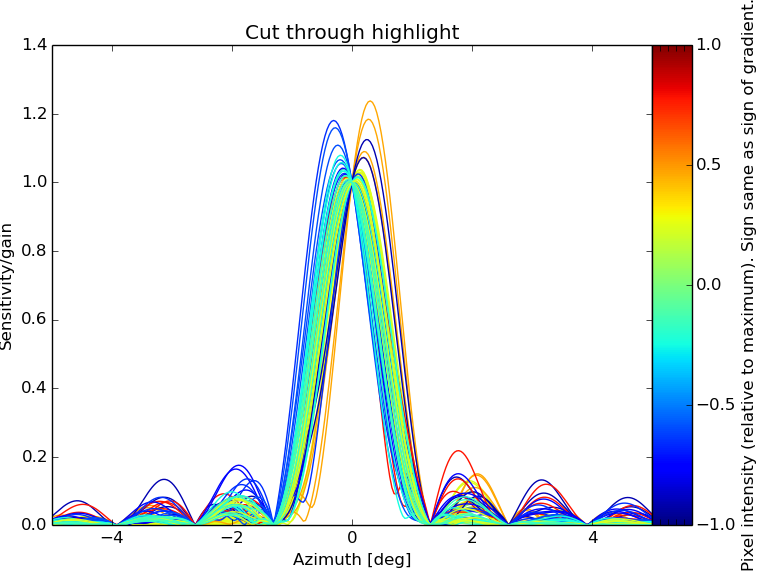
\includegraphics[width=0.49\linewidth]{gfx/3_win_resp_cut_highlight.png}}\\
\end{narrow}
\end{figure*}
\newpage
\begin{figure*}[!t]
\begin{narrow}{-1.2cm}{-1.2cm}\centering\vspace{-1.0cm}
\textbf{4. Capon: Tuning subarray.}\\
\begin{tabular}[c]{l l l l}
\bf General & M = 32                            & $\Delta r = \frac{c}{2B}$ = 2.5 cm & $\frac{640\,\text{pixels}] / 12\,\text{m}}{\Delta r} = \frac{4}{3}$ \\
\bf LCA     & $\beta \in [0,10]$ (9 values) & $\phi \in [-1.07,1.07]$ deg (9 values) & Navg = 3 \\
\bf Capon   & $\Delta$ = 0.01                 & L = 20                           & Navg = 3 \\
\end{tabular}
\subfloat[LCA Window Response]{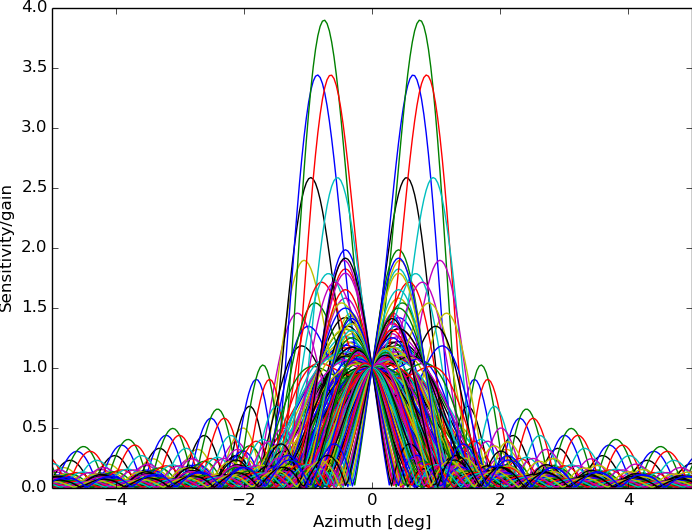
\includegraphics[width=0.49\linewidth]{gfx/4_window_response.png}}\hfill
\subfloat[Mean images]{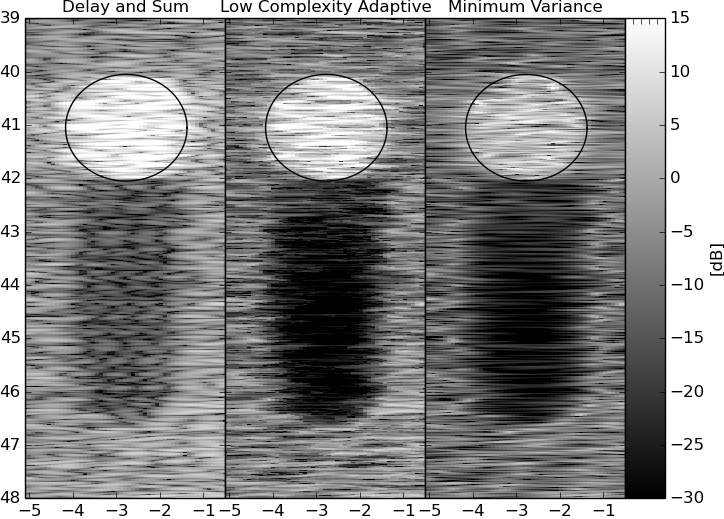
\includegraphics[width=0.49\linewidth]{gfx/4_mean_imgs.png}}\\
\subfloat[Windows ($\beta$)]{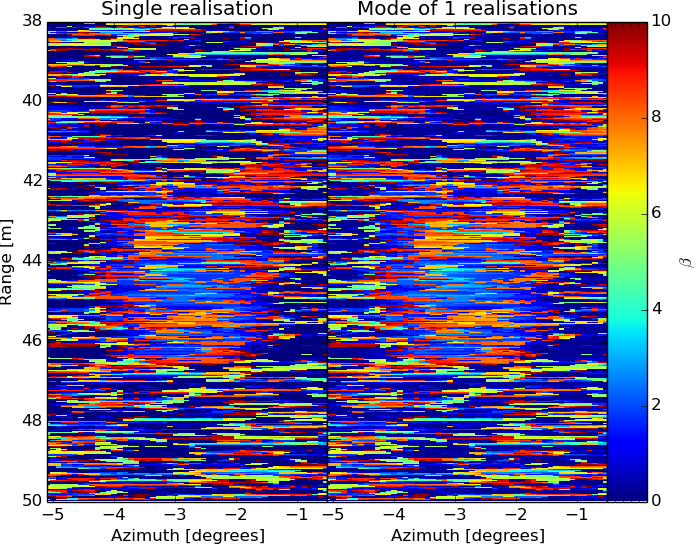
\includegraphics[width=0.49\linewidth]{gfx/4_windows_beta.png}}\hfill
\subfloat[Windows ($\phi$)]{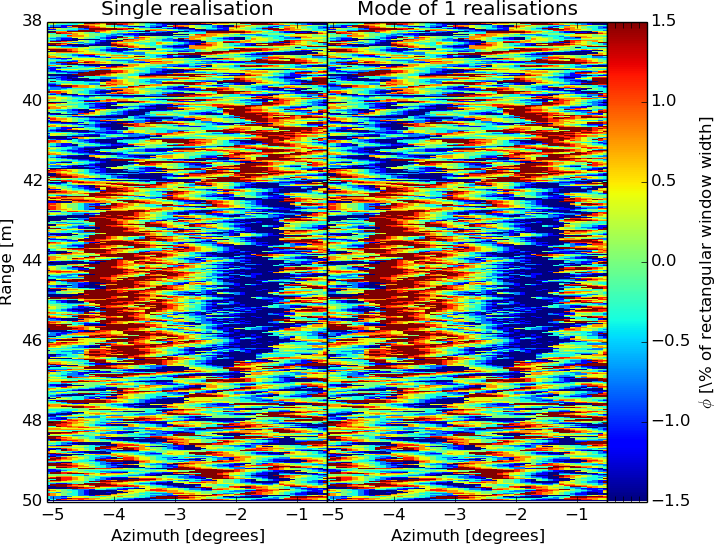
\includegraphics[width=0.48\linewidth]{gfx/4_windows_phi.png}}\\
\subfloat[Capon win. resp. through shadow]{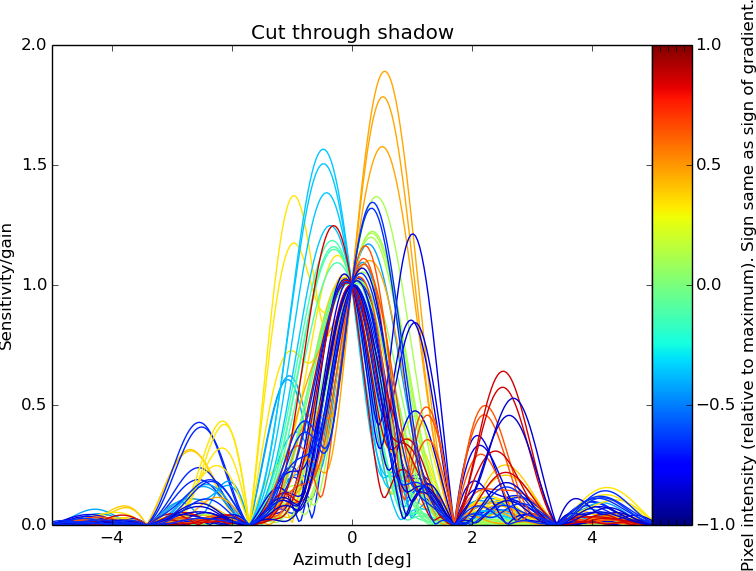
\includegraphics[width=0.49\linewidth]{gfx/4_win_resp_cut_shadow.png}}\hfill
\subfloat[Capon win. resp. through highlight]{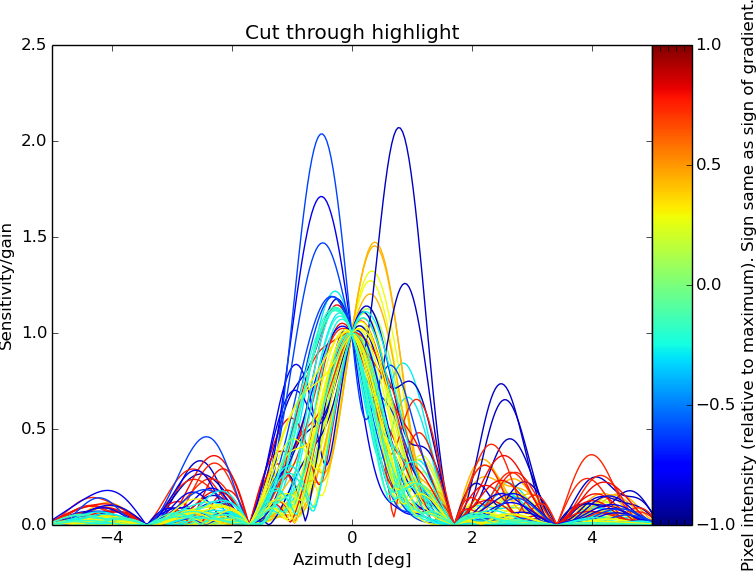
\includegraphics[width=0.49\linewidth]{gfx/4_win_resp_cut_highlight.png}}\\
\end{narrow}
\end{figure*}
\newpage
\begin{figure*}[!t]
\begin{narrow}{-1.2cm}{-1.2cm}\centering\vspace{-1.0cm}
\textbf{5. Capon: Tuning subarray.}\\
\begin{tabular}[c]{l l l l}
\bf General & M = 32                            & $\Delta r = \frac{c}{2B}$ = 2.5 cm & $\frac{640\,\text{pixels}] / 12\,\text{m}}{\Delta r} = \frac{4}{3}$ \\
\bf LCA     & $\beta \in [0,10]$ (9 values) & $\phi \in [-1.07,1.07]$ deg (9 values) & Navg = 3 \\
\bf Capon   & $\Delta$ = 0.01                 & L = 16                           & Navg = 3 \\
\end{tabular}
\subfloat[LCA Window Response]{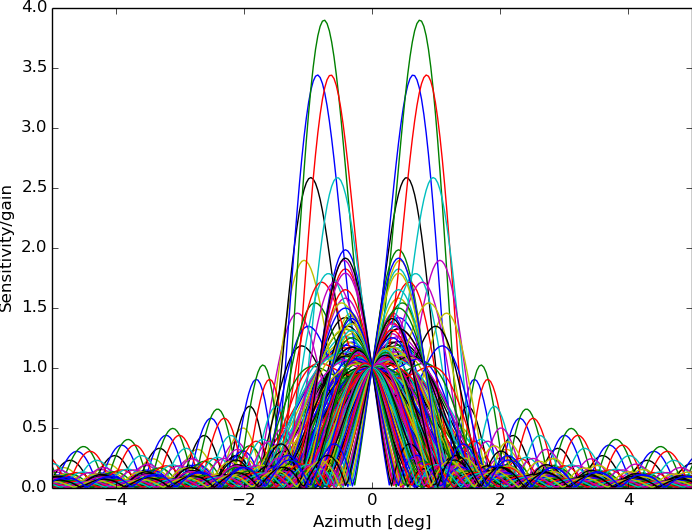
\includegraphics[width=0.49\linewidth]{gfx/5_window_response.png}}\hfill
\subfloat[Mean images]{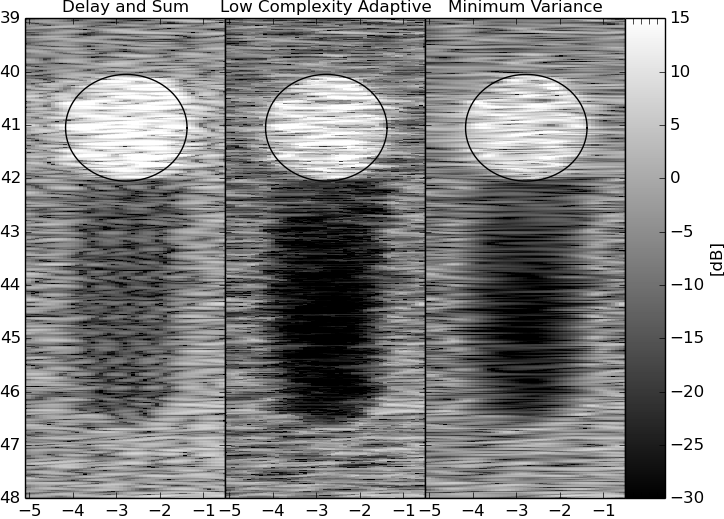
\includegraphics[width=0.49\linewidth]{gfx/5_mean_imgs.png}}\\
\subfloat[Windows ($\beta$)]{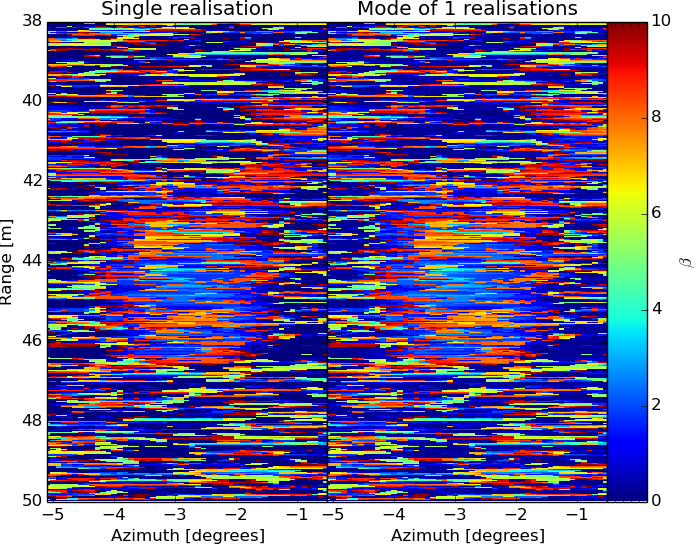
\includegraphics[width=0.49\linewidth]{gfx/5_windows_beta.png}}\hfill
\subfloat[Windows ($\phi$)]{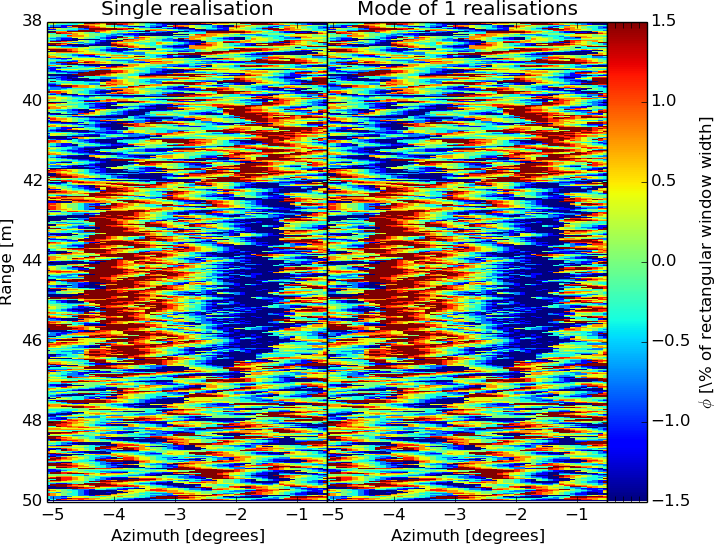
\includegraphics[width=0.48\linewidth]{gfx/5_windows_phi.png}}\\
\subfloat[Capon win. resp. through shadow]{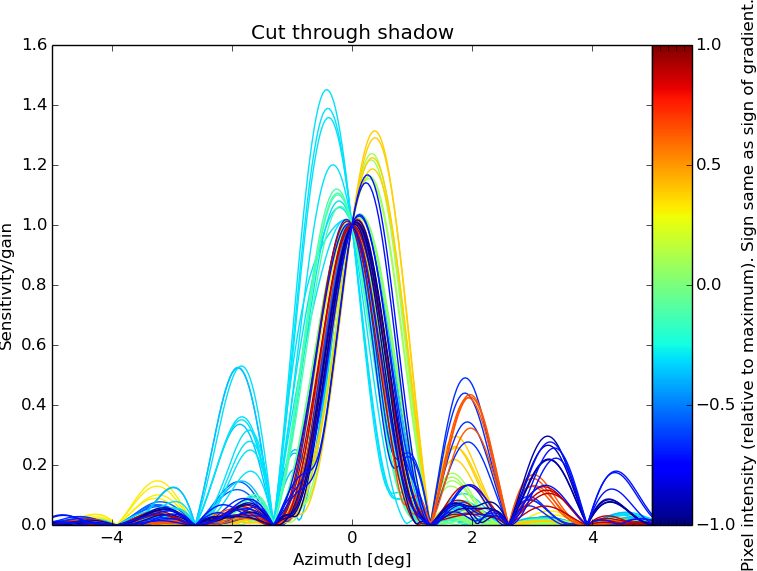
\includegraphics[width=0.49\linewidth]{gfx/5_win_resp_cut_shadow.png}}\hfill
\subfloat[Capon win. resp. through highlight]{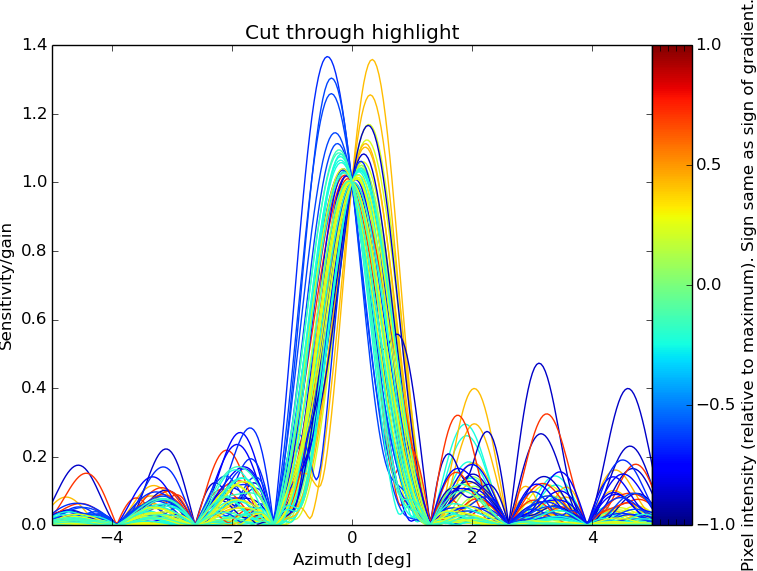
\includegraphics[width=0.49\linewidth]{gfx/5_win_resp_cut_highlight.png}}\\
\end{narrow}
\end{figure*}
\newpage
\begin{figure*}[!t]
\begin{narrow}{-1.2cm}{-1.2cm}\centering\vspace{-1.0cm}
\textbf{6. Capon: Tuning subarray.}\\
\begin{tabular}[c]{l l l l}
\bf General & M = 32                            & $\Delta r = \frac{c}{2B}$ = 2.5 cm & $\frac{640\,\text{pixels}] / 12\,\text{m}}{\Delta r} = \frac{4}{3}$ \\
\bf LCA     & $\beta \in [0,10]$ (9 values) & $\phi \in [-1.07,1.07]$ deg (9 values) & Navg = 3 \\
\bf Capon   & $\Delta$ = 0.01                 & L = 12                           & Navg = 3 \\
\end{tabular}
\subfloat[LCA Window Response]{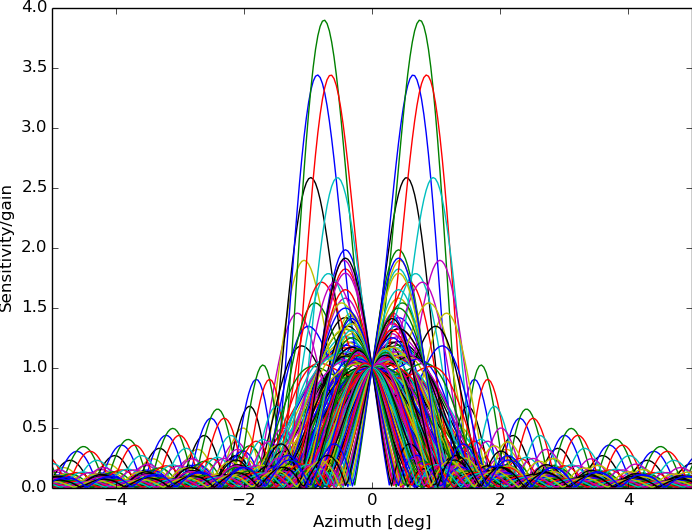
\includegraphics[width=0.49\linewidth]{gfx/6_window_response.png}}\hfill
\subfloat[Mean images]{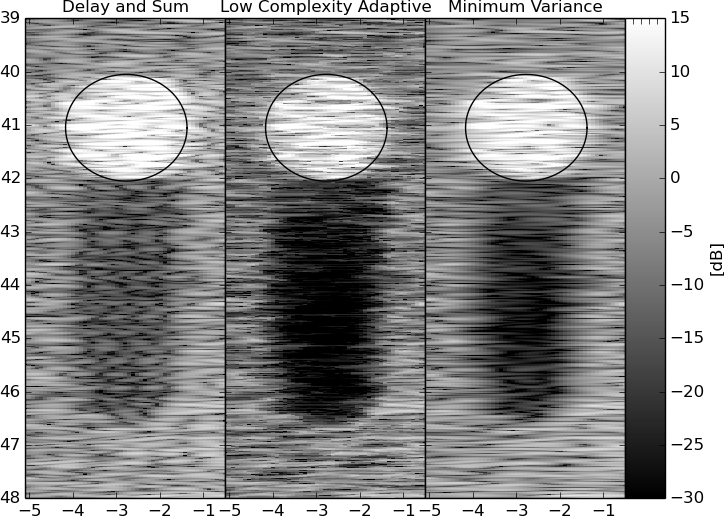
\includegraphics[width=0.49\linewidth]{gfx/6_mean_imgs.png}}\\
\subfloat[Windows ($\beta$)]{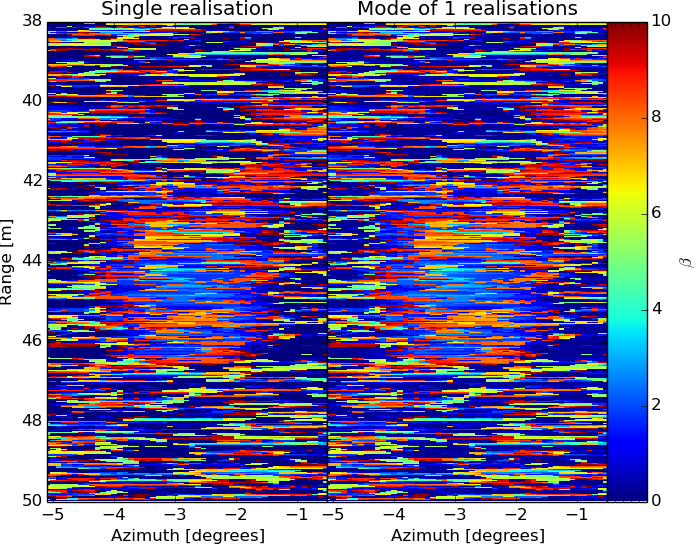
\includegraphics[width=0.49\linewidth]{gfx/6_windows_beta.png}}\hfill
\subfloat[Windows ($\phi$)]{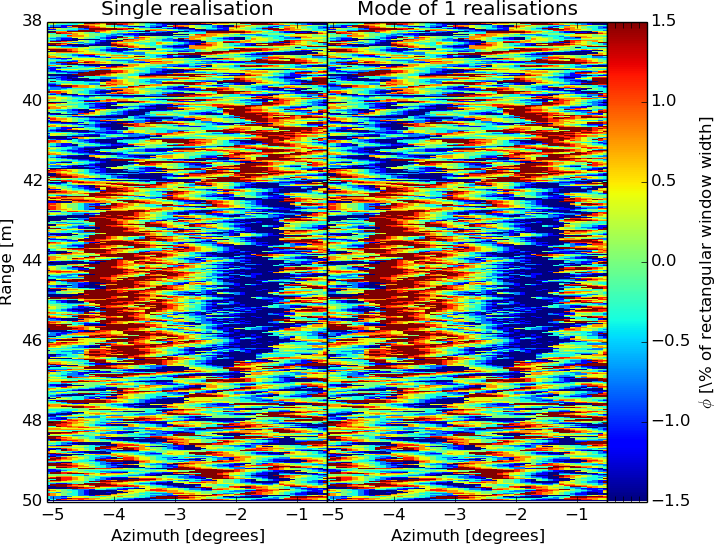
\includegraphics[width=0.48\linewidth]{gfx/6_windows_phi.png}}\\
\subfloat[Capon win. resp. through shadow]{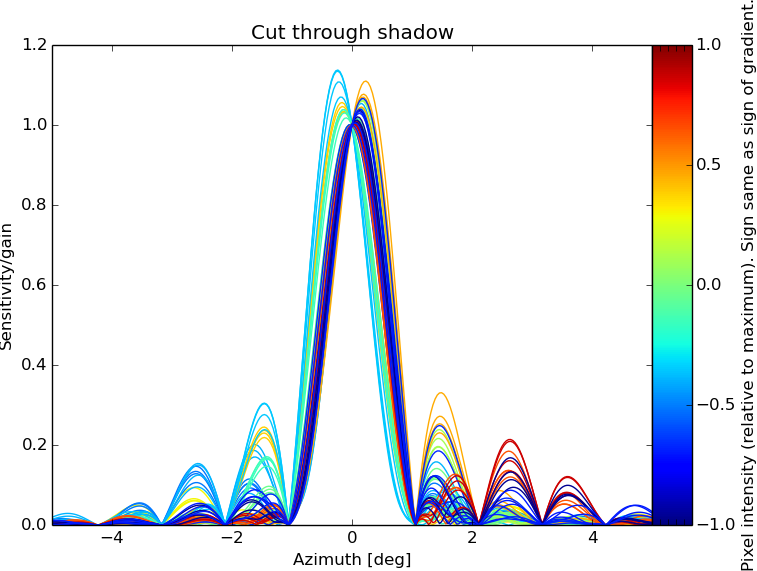
\includegraphics[width=0.49\linewidth]{gfx/6_win_resp_cut_shadow.png}}\hfill
\subfloat[Capon win. resp. through highlight]{\includegraphics[width=0.49\linewidth]{gfx/6_win_resp_cut_highlight.png}}\\
\end{narrow}
\end{figure*}
\newpage
\begin{figure*}[!t]
\begin{narrow}{-1.2cm}{-1.2cm}\centering\vspace{-1.0cm}
\textbf{7. Capon: Tuning time averaging.}\\
\begin{tabular}[c]{l l l l}
\bf General & M = 32                            & $\Delta r = \frac{c}{2B}$ = 2.5 cm & $\frac{640\,\text{pixels}] / 12\,\text{m}}{\Delta r} = \frac{4}{3}$ \\
\bf LCA     & $\beta \in [0,10]$ (9 values) & $\phi \in [-1.07,1.07]$ deg (9 values) & Navg = 1 \\
\bf Capon   & $\Delta$ = 0.01                 & L = 16                           & Navg = 1 \\
\end{tabular}
\subfloat[LCA Window Response]{\includegraphics[width=0.49\linewidth]{gfx/7_window_response.png}}\hfill
\subfloat[Mean images]{\includegraphics[width=0.49\linewidth]{gfx/7_mean_imgs.png}}\\
\subfloat[Windows ($\beta$)]{\includegraphics[width=0.49\linewidth]{gfx/7_windows_beta.png}}\hfill
\subfloat[Windows ($\phi$)]{\includegraphics[width=0.48\linewidth]{gfx/7_windows_phi.png}}\\
\subfloat[Capon win. resp. through shadow]{\includegraphics[width=0.49\linewidth]{gfx/7_win_resp_cut_shadow.png}}\hfill
\subfloat[Capon win. resp. through highlight]{\includegraphics[width=0.49\linewidth]{gfx/7_win_resp_cut_highlight.png}}\\
\end{narrow}
\end{figure*}
\newpage
\begin{figure*}[!t]
\begin{narrow}{-1.2cm}{-1.2cm}\centering\vspace{-1.0cm}
\textbf{8. Capon: Tuning time averaging.}\\
\begin{tabular}[c]{l l l l}
\bf General & M = 32                            & $\Delta r = \frac{c}{2B}$ = 2.5 cm & $\frac{640\,\text{pixels}] / 12\,\text{m}}{\Delta r} = \frac{4}{3}$ \\
\bf LCA     & $\beta \in [0,10]$ (9 values) & $\phi \in [-1.07,1.07]$ deg (9 values) & Navg = 3 \\
\bf Capon   & $\Delta$ = 0.01                 & L = 16                           & Navg = 3 \\
\end{tabular}
\subfloat[LCA Window Response]{\includegraphics[width=0.49\linewidth]{gfx/8_window_response.png}}\hfill
\subfloat[Mean images]{\includegraphics[width=0.49\linewidth]{gfx/8_mean_imgs.png}}\\
\subfloat[Windows ($\beta$)]{\includegraphics[width=0.49\linewidth]{gfx/8_windows_beta.png}}\hfill
\subfloat[Windows ($\phi$)]{\includegraphics[width=0.48\linewidth]{gfx/8_windows_phi.png}}\\
\subfloat[Capon win. resp. through shadow]{\includegraphics[width=0.49\linewidth]{gfx/8_win_resp_cut_shadow.png}}\hfill
\subfloat[Capon win. resp. through highlight]{\includegraphics[width=0.49\linewidth]{gfx/8_win_resp_cut_highlight.png}}\\
\end{narrow}
\end{figure*}
\newpage
\begin{figure*}[!t]
\begin{narrow}{-1.2cm}{-1.2cm}\centering\vspace{-1.0cm}
\textbf{9. Capon: Tuning time averaging.}\\
\begin{tabular}[c]{l l l l}
\bf General & M = 32                            & $\Delta r = \frac{c}{2B}$ = 2.5 cm & $\frac{640\,\text{pixels}] / 12\,\text{m}}{\Delta r} = \frac{4}{3}$ \\
\bf LCA     & $\beta \in [0,10]$ (9 values) & $\phi \in [-1.07,1.07]$ deg (9 values) & Navg = 5 \\
\bf Capon   & $\Delta$ = 0.01                 & L = 16                           & Navg = 5 \\
\end{tabular}
\subfloat[LCA Window Response]{\includegraphics[width=0.49\linewidth]{gfx/9_window_response.png}}\hfill
\subfloat[Mean images]{\includegraphics[width=0.49\linewidth]{gfx/9_mean_imgs.png}}\\
\subfloat[Windows ($\beta$)]{\includegraphics[width=0.49\linewidth]{gfx/9_windows_beta.png}}\hfill
\subfloat[Windows ($\phi$)]{\includegraphics[width=0.48\linewidth]{gfx/9_windows_phi.png}}\\
\subfloat[Capon win. resp. through shadow]{\includegraphics[width=0.49\linewidth]{gfx/9_win_resp_cut_shadow.png}}\hfill
\subfloat[Capon win. resp. through highlight]{\includegraphics[width=0.49\linewidth]{gfx/9_win_resp_cut_highlight.png}}\\
\end{narrow}
\end{figure*}
\newpage
\begin{figure*}[!t]
\begin{narrow}{-1.2cm}{-1.2cm}\centering\vspace{-1.0cm}
\textbf{10. Capon: Tuning time averaging.}\\
\begin{tabular}[c]{l l l l}
\bf General & M = 32                            & $\Delta r = \frac{c}{2B}$ = 2.5 cm & $\frac{640\,\text{pixels}] / 12\,\text{m}}{\Delta r} = \frac{4}{3}$ \\
\bf LCA     & $\beta \in [0,10]$ (9 values) & $\phi \in [-1.07,1.07]$ deg (9 values) & Navg = 7 \\
\bf Capon   & $\Delta$ = 0.01                 & L = 16                           & Navg = 7 \\
\end{tabular}
\subfloat[LCA Window Response]{\includegraphics[width=0.49\linewidth]{gfx/10_window_response.png}}\hfill
\subfloat[Mean images]{\includegraphics[width=0.49\linewidth]{gfx/10_mean_imgs.png}}\\
\subfloat[Windows ($\beta$)]{\includegraphics[width=0.49\linewidth]{gfx/10_windows_beta.png}}\hfill
\subfloat[Windows ($\phi$)]{\includegraphics[width=0.48\linewidth]{gfx/10_windows_phi.png}}\\
\subfloat[Capon win. resp. through shadow]{\includegraphics[width=0.49\linewidth]{gfx/10_win_resp_cut_shadow.png}}\hfill
\subfloat[Capon win. resp. through highlight]{\includegraphics[width=0.49\linewidth]{gfx/10_win_resp_cut_highlight.png}}\\
\end{narrow}
\end{figure*}
\newpage
\begin{figure*}[!t]
\begin{narrow}{-1.2cm}{-1.2cm}\centering\vspace{-1.0cm}
\textbf{11. LCA: Reasonable settings.}\\
\begin{tabular}[c]{l l l l}
\bf General & M = 32                            & $\Delta r = \frac{c}{2B}$ = 2.5 cm & $\frac{640\,\text{pixels}] / 12\,\text{m}}{\Delta r} = \frac{4}{3}$ \\
\bf LCA     & $\beta \in [0,10]$ (9 values) & $\phi \in [-0.57,0.57]$ deg (9 values) & Navg = 7 \\
\bf Capon   & $\Delta$ = 0.01                 & L = 16                           & Navg = 7 \\
\end{tabular}
\subfloat[LCA Window Response]{\includegraphics[width=0.49\linewidth]{gfx/11_window_response.png}}\hfill
\subfloat[Mean images]{\includegraphics[width=0.49\linewidth]{gfx/11_mean_imgs.png}}\\
\subfloat[Windows ($\beta$)]{\includegraphics[width=0.49\linewidth]{gfx/11_windows_beta.png}}\hfill
\subfloat[Windows ($\phi$)]{\includegraphics[width=0.48\linewidth]{gfx/11_windows_phi.png}}\\
\subfloat[Capon win. resp. through shadow]{\includegraphics[width=0.49\linewidth]{gfx/11_win_resp_cut_shadow.png}}\hfill
\subfloat[Capon win. resp. through highlight]{\includegraphics[width=0.49\linewidth]{gfx/11_win_resp_cut_highlight.png}}\\
\end{narrow}
\end{figure*}
\newpage
\begin{figure*}[!t]
\begin{narrow}{-1.2cm}{-1.2cm}\centering\vspace{-1.0cm}
\textbf{12. LCA: Lots of Kaiser windows - wide span.}\\
\begin{tabular}[c]{l l l l}
\bf General & M = 32                            & $\Delta r = \frac{c}{2B}$ = 2.5 cm & $\frac{640\,\text{pixels}] / 12\,\text{m}}{\Delta r} = \frac{4}{3}$ \\
\bf LCA     & $\beta \in [0,20]$ (19 values) & $\phi \in [-1.07,1.07]$ deg (19 values) & Navg = 7 \\
\bf Capon   & $\Delta$ = 0.01                 & L = 16                           & Navg = 7 \\
\end{tabular}
\subfloat[LCA Window Response]{\includegraphics[width=0.49\linewidth]{gfx/12_window_response.png}}\hfill
\subfloat[Mean images]{\includegraphics[width=0.49\linewidth]{gfx/12_mean_imgs.png}}\\
\subfloat[Windows ($\beta$)]{\includegraphics[width=0.49\linewidth]{gfx/12_windows_beta.png}}\hfill
\subfloat[Windows ($\phi$)]{\includegraphics[width=0.48\linewidth]{gfx/12_windows_phi.png}}\\
\subfloat[Capon win. resp. through shadow]{\includegraphics[width=0.49\linewidth]{gfx/12_win_resp_cut_shadow.png}}\hfill
\subfloat[Capon win. resp. through highlight]{\includegraphics[width=0.49\linewidth]{gfx/12_win_resp_cut_highlight.png}}\\
\end{narrow}
\end{figure*}
\newpage
\begin{figure*}[!t]
\begin{narrow}{-1.2cm}{-1.2cm}\centering\vspace{-1.0cm}
\textbf{13. LCA: Lots of trigonometric windows - wide span.}\\
\begin{tabular}[c]{l l l l}
\bf General & M = 32                            & $\Delta r = \frac{c}{2B}$ = 2.5 cm & $\frac{640\,\text{pixels}] / 12\,\text{m}}{\Delta r} = \frac{4}{3}$ \\
\bf LCA     & $\beta \in [0,20]$ (19 values) & $\phi \in [-1.07,1.07]$ deg (19 values) & Navg = 7 \\
\bf Capon   & $\Delta$ = 0.01                 & L = 16                           & Navg = 7 \\
\end{tabular}
\subfloat[LCA Window Response]{\includegraphics[width=0.49\linewidth]{gfx/13_window_response.png}}\hfill
\subfloat[Mean images]{\includegraphics[width=0.49\linewidth]{gfx/13_mean_imgs.png}}\\
\subfloat[Windows ($\beta$)]{\includegraphics[width=0.49\linewidth]{gfx/13_windows_beta.png}}\hfill
\subfloat[Windows ($\phi$)]{\includegraphics[width=0.48\linewidth]{gfx/13_windows_phi.png}}\\
\subfloat[Capon win. resp. through shadow]{\includegraphics[width=0.49\linewidth]{gfx/13_win_resp_cut_shadow.png}}\hfill
\subfloat[Capon win. resp. through highlight]{\includegraphics[width=0.49\linewidth]{gfx/13_win_resp_cut_highlight.png}}\\
\end{narrow}
\end{figure*}
\newpage
\begin{figure*}[!t]
\begin{narrow}{-1.2cm}{-1.2cm}\centering\vspace{-1.0cm}
\textbf{14. LCA: Back on Kaiser - reducing steering span.}\\
\begin{tabular}[c]{l l l l}
\bf General & M = 32                            & $\Delta r = \frac{c}{2B}$ = 2.5 cm & $\frac{640\,\text{pixels}] / 12\,\text{m}}{\Delta r} = \frac{4}{3}$ \\
\bf LCA     & $\beta \in [0,20]$ (19 values) & $\phi \in [-0.72,0.72]$ deg (19 values) & Navg = 7 \\
\bf Capon   & $\Delta$ = 0.01                 & L = 16                           & Navg = 7 \\
\end{tabular}
\subfloat[LCA Window Response]{\includegraphics[width=0.49\linewidth]{gfx/14_window_response.png}}\hfill
\subfloat[Mean images]{\includegraphics[width=0.49\linewidth]{gfx/14_mean_imgs.png}}\\
\subfloat[Windows ($\beta$)]{\includegraphics[width=0.49\linewidth]{gfx/14_windows_beta.png}}\hfill
\subfloat[Windows ($\phi$)]{\includegraphics[width=0.48\linewidth]{gfx/14_windows_phi.png}}\\
\subfloat[Capon win. resp. through shadow]{\includegraphics[width=0.49\linewidth]{gfx/14_win_resp_cut_shadow.png}}\hfill
\subfloat[Capon win. resp. through highlight]{\includegraphics[width=0.49\linewidth]{gfx/14_win_resp_cut_highlight.png}}\\
\end{narrow}
\end{figure*}
\newpage
\begin{figure*}[!t]
\begin{narrow}{-1.2cm}{-1.2cm}\centering\vspace{-1.0cm}
\textbf{15. LCA: Reducing steering span.}\\
\begin{tabular}[c]{l l l l}
\bf General & M = 32                            & $\Delta r = \frac{c}{2B}$ = 2.5 cm & $\frac{640\,\text{pixels}] / 12\,\text{m}}{\Delta r} = \frac{4}{3}$ \\
\bf LCA     & $\beta \in [0,20]$ (19 values) & $\phi \in [-0.36,0.36]$ deg (19 values) & Navg = 7 \\
\bf Capon   & $\Delta$ = 0.01                 & L = 16                           & Navg = 7 \\
\end{tabular}
\subfloat[LCA Window Response]{\includegraphics[width=0.49\linewidth]{gfx/15_window_response.png}}\hfill
\subfloat[Mean images]{\includegraphics[width=0.49\linewidth]{gfx/15_mean_imgs.png}}\\
\subfloat[Windows ($\beta$)]{\includegraphics[width=0.49\linewidth]{gfx/15_windows_beta.png}}\hfill
\subfloat[Windows ($\phi$)]{\includegraphics[width=0.48\linewidth]{gfx/15_windows_phi.png}}\\
\subfloat[Capon win. resp. through shadow]{\includegraphics[width=0.49\linewidth]{gfx/15_win_resp_cut_shadow.png}}\hfill
\subfloat[Capon win. resp. through highlight]{\includegraphics[width=0.49\linewidth]{gfx/15_win_resp_cut_highlight.png}}\\
\end{narrow}
\end{figure*}
\newpage
\begin{figure*}[!t]
\begin{narrow}{-1.2cm}{-1.2cm}\centering\vspace{-1.0cm}
\textbf{16. LCA: Adjusting resolution/SNR.}\\
\begin{tabular}[c]{l l l l}
\bf General & M = 32                            & $\Delta r = \frac{c}{2B}$ = 2.5 cm & $\frac{640\,\text{pixels}] / 12\,\text{m}}{\Delta r} = \frac{4}{3}$ \\
\bf LCA     & $\beta \in [0,5]$ (19 values) & $\phi \in [-0.72,0.72]$ deg (19 values) & Navg = 7 \\
\bf Capon   & $\Delta$ = 0.01                 & L = 16                           & Navg = 7 \\
\end{tabular}
\subfloat[LCA Window Response]{\includegraphics[width=0.49\linewidth]{gfx/16_window_response.png}}\hfill
\subfloat[Mean images]{\includegraphics[width=0.49\linewidth]{gfx/16_mean_imgs.png}}\\
\subfloat[Windows ($\beta$)]{\includegraphics[width=0.49\linewidth]{gfx/16_windows_beta.png}}\hfill
\subfloat[Windows ($\phi$)]{\includegraphics[width=0.48\linewidth]{gfx/16_windows_phi.png}}\\
\subfloat[Capon win. resp. through shadow]{\includegraphics[width=0.49\linewidth]{gfx/16_win_resp_cut_shadow.png}}\hfill
\subfloat[Capon win. resp. through highlight]{\includegraphics[width=0.49\linewidth]{gfx/16_win_resp_cut_highlight.png}}\\
\end{narrow}
\end{figure*}
\newpage
\begin{figure*}[!t]
\begin{narrow}{-1.2cm}{-1.2cm}\centering\vspace{-1.0cm}
\textbf{17. LCA: Adjusting resolution/SNR.}\\
\begin{tabular}[c]{l l l l}
\bf General & M = 32                            & $\Delta r = \frac{c}{2B}$ = 2.5 cm & $\frac{640\,\text{pixels}] / 12\,\text{m}}{\Delta r} = \frac{4}{3}$ \\
\bf LCA     & $\beta \in [5,20]$ (19 values) & $\phi \in [-0.72,0.72]$ deg (19 values) & Navg = 7 \\
\bf Capon   & $\Delta$ = 0.01                 & L = 16                           & Navg = 7 \\
\end{tabular}
\subfloat[LCA Window Response]{\includegraphics[width=0.49\linewidth]{gfx/17_window_response.png}}\hfill
\subfloat[Mean images]{\includegraphics[width=0.49\linewidth]{gfx/17_mean_imgs.png}}\\
\subfloat[Windows ($\beta$)]{\includegraphics[width=0.49\linewidth]{gfx/17_windows_beta.png}}\hfill
\subfloat[Windows ($\phi$)]{\includegraphics[width=0.48\linewidth]{gfx/17_windows_phi.png}}\\
\subfloat[Capon win. resp. through shadow]{\includegraphics[width=0.49\linewidth]{gfx/17_win_resp_cut_shadow.png}}\hfill
\subfloat[Capon win. resp. through highlight]{\includegraphics[width=0.49\linewidth]{gfx/17_win_resp_cut_highlight.png}}\\
\end{narrow}
\end{figure*}
\newpage
\begin{figure*}[!t]
\begin{narrow}{-1.2cm}{-1.2cm}\centering\vspace{-1.0cm}
\textbf{18. LCA: Fewer windows.}\\
\begin{tabular}[c]{l l l l}
\bf General & M = 32                            & $\Delta r = \frac{c}{2B}$ = 2.5 cm & $\frac{640\,\text{pixels}] / 12\,\text{m}}{\Delta r} = \frac{4}{3}$ \\
\bf LCA     & $\beta \in [0,10]$ (9 values) & $\phi \in [-0.72,0.72]$ deg (19 values) & Navg = 7 \\
\bf Capon   & $\Delta$ = 0.01                 & L = 16                           & Navg = 7 \\
\end{tabular}
\subfloat[LCA Window Response]{\includegraphics[width=0.49\linewidth]{gfx/18_window_response.png}}\hfill
\subfloat[Mean images]{\includegraphics[width=0.49\linewidth]{gfx/18_mean_imgs.png}}\\
\subfloat[Windows ($\beta$)]{\includegraphics[width=0.49\linewidth]{gfx/18_windows_beta.png}}\hfill
\subfloat[Windows ($\phi$)]{\includegraphics[width=0.48\linewidth]{gfx/18_windows_phi.png}}\\
\subfloat[Capon win. resp. through shadow]{\includegraphics[width=0.49\linewidth]{gfx/18_win_resp_cut_shadow.png}}\hfill
\subfloat[Capon win. resp. through highlight]{\includegraphics[width=0.49\linewidth]{gfx/18_win_resp_cut_highlight.png}}\\
\end{narrow}
\end{figure*}
\newpage
\begin{figure*}[!t]
\begin{narrow}{-1.2cm}{-1.2cm}\centering\vspace{-1.0cm}
\textbf{19. LCA: Fewer steering angles.}\\
\begin{tabular}[c]{l l l l}
\bf General & M = 32                            & $\Delta r = \frac{c}{2B}$ = 2.5 cm & $\frac{640\,\text{pixels}] / 12\,\text{m}}{\Delta r} = \frac{4}{3}$ \\
\bf LCA     & $\beta \in [0,10]$ (19 values) & $\phi \in [-0.72,0.72]$ deg (9 values) & Navg = 7 \\
\bf Capon   & $\Delta$ = 0.01                 & L = 16                           & Navg = 7 \\
\end{tabular}
\subfloat[LCA Window Response]{\includegraphics[width=0.49\linewidth]{gfx/19_window_response.png}}\hfill
\subfloat[Mean images]{\includegraphics[width=0.49\linewidth]{gfx/19_mean_imgs.png}}\\
\subfloat[Windows ($\beta$)]{\includegraphics[width=0.49\linewidth]{gfx/19_windows_beta.png}}\hfill
\subfloat[Windows ($\phi$)]{\includegraphics[width=0.48\linewidth]{gfx/19_windows_phi.png}}\\
\subfloat[Capon win. resp. through shadow]{\includegraphics[width=0.49\linewidth]{gfx/19_win_resp_cut_shadow.png}}\hfill
\subfloat[Capon win. resp. through highlight]{\includegraphics[width=0.49\linewidth]{gfx/19_win_resp_cut_highlight.png}}\\
\end{narrow}
\end{figure*}
\newpage
\begin{figure*}[!t]
\begin{narrow}{-1.2cm}{-1.2cm}\centering\vspace{-1.0cm}
\textbf{20. LCA: Fewer both.}\\
\begin{tabular}[c]{l l l l}
\bf General & M = 32                            & $\Delta r = \frac{c}{2B}$ = 2.5 cm & $\frac{640\,\text{pixels}] / 12\,\text{m}}{\Delta r} = \frac{4}{3}$ \\
\bf LCA     & $\beta \in [0,10]$ (9 values) & $\phi \in [-0.72,0.72]$ deg (9 values) & Navg = 7 \\
\bf Capon   & $\Delta$ = 0.01                 & L = 16                           & Navg = 7 \\
\end{tabular}
\subfloat[LCA Window Response]{\includegraphics[width=0.49\linewidth]{gfx/20_window_response.png}}\hfill
\subfloat[Mean images]{\includegraphics[width=0.49\linewidth]{gfx/20_mean_imgs.png}}\\
\subfloat[Windows ($\beta$)]{\includegraphics[width=0.49\linewidth]{gfx/20_windows_beta.png}}\hfill
\subfloat[Windows ($\phi$)]{\includegraphics[width=0.48\linewidth]{gfx/20_windows_phi.png}}\\
\subfloat[Capon win. resp. through shadow]{\includegraphics[width=0.49\linewidth]{gfx/20_win_resp_cut_shadow.png}}\hfill
\subfloat[Capon win. resp. through highlight]{\includegraphics[width=0.49\linewidth]{gfx/20_win_resp_cut_highlight.png}}\\
\end{narrow}
\end{figure*}
\newpage
\begin{figure*}[!t]
\begin{narrow}{-1.2cm}{-1.2cm}\centering\vspace{-1.0cm}
\textbf{21. LCA: Even less.}\\
\begin{tabular}[c]{l l l l}
\bf General & M = 32                            & $\Delta r = \frac{c}{2B}$ = 2.5 cm & $\frac{640\,\text{pixels}] / 12\,\text{m}}{\Delta r} = \frac{4}{3}$ \\
\bf LCA     & $\beta \in [0,5]$ (9 values) & $\phi \in [-0.72,0.72]$ deg (5 values) & Navg = 7 \\
\bf Capon   & $\Delta$ = 0.01                 & L = 16                           & Navg = 7 \\
\end{tabular}
\subfloat[LCA Window Response]{\includegraphics[width=0.49\linewidth]{gfx/21_window_response.png}}\hfill
\subfloat[Mean images]{\includegraphics[width=0.49\linewidth]{gfx/21_mean_imgs.png}}\\
\subfloat[Windows ($\beta$)]{\includegraphics[width=0.49\linewidth]{gfx/21_windows_beta.png}}\hfill
\subfloat[Windows ($\phi$)]{\includegraphics[width=0.48\linewidth]{gfx/21_windows_phi.png}}\\
\subfloat[Capon win. resp. through shadow]{\includegraphics[width=0.49\linewidth]{gfx/21_win_resp_cut_shadow.png}}\hfill
\subfloat[Capon win. resp. through highlight]{\includegraphics[width=0.49\linewidth]{gfx/21_win_resp_cut_highlight.png}}\\
\end{narrow}
\end{figure*}
\newpage
\begin{figure*}[!t]
\begin{narrow}{-1.2cm}{-1.2cm}\centering\vspace{-1.0cm}
\textbf{22. LCA: Hardly any.}\\
\begin{tabular}[c]{l l l l}
\bf General & M = 32                            & $\Delta r = \frac{c}{2B}$ = 2.5 cm & $\frac{640\,\text{pixels}] / 12\,\text{m}}{\Delta r} = \frac{4}{3}$ \\
\bf LCA     & $\beta \in [0,5]$ (5 values) & $\phi \in [-0.72,0.72]$ deg (5 values) & Navg = 7 \\
\bf Capon   & $\Delta$ = 0.01                 & L = 16                           & Navg = 7 \\
\end{tabular}
\subfloat[LCA Window Response]{\includegraphics[width=0.49\linewidth]{gfx/22_window_response.png}}\hfill
\subfloat[Mean images]{\includegraphics[width=0.49\linewidth]{gfx/22_mean_imgs.png}}\\
\subfloat[Windows ($\beta$)]{\includegraphics[width=0.49\linewidth]{gfx/22_windows_beta.png}}\hfill
\subfloat[Windows ($\phi$)]{\includegraphics[width=0.48\linewidth]{gfx/22_windows_phi.png}}\\
\subfloat[Capon win. resp. through shadow]{\includegraphics[width=0.49\linewidth]{gfx/22_win_resp_cut_shadow.png}}\hfill
\subfloat[Capon win. resp. through highlight]{\includegraphics[width=0.49\linewidth]{gfx/22_win_resp_cut_highlight.png}}\\
\end{narrow}
\end{figure*}


\end{document}


